% !TeX root = ./thesis.tex
% !TeX encoding = UTF-8
% !TeX spellcheck = en_GB


\documentclass[oneside]{mystyle}

% Set up metadata
\author{Wouter Duverger}
\title{Polarisation-resolved super-resolution microscopy}
\date{May 10, 2021}

% Register figure folders (twice, for Windows and Linux)
\graphicspath{
	{../figures_generated}
	{../figures_generated/}
	{../figures_other}
	{../figures_other/}
}

% Shorthands
\newcommand{\qwp}{{\lambda/4}}
\newcommand{\hwp}{{\lambda/2}}
\newcommand{\Eox}{E_{0x}}
\newcommand{\Eoy}{E_{0y}}
\newcommand{\na}{\mathrm{NA}}
\newcommand{\exc}{\mathit{ex}}
\newcommand{\dep}{\mathit{d}}
\newcommand{\emm}{\mathit{em}}
\newcommand{\unit}[1]{\hat{\vb{#1}}}
\newcommand{\se}{\mathit{se}}

%\includeonly{text/methods}

\begin{document}

% !TeX spellcheck = en_GB
{
\pagestyle{empty}

\begin{tikzpicture}[remember picture,overlay]
	\node[inner sep=0pt] at (current page.center) {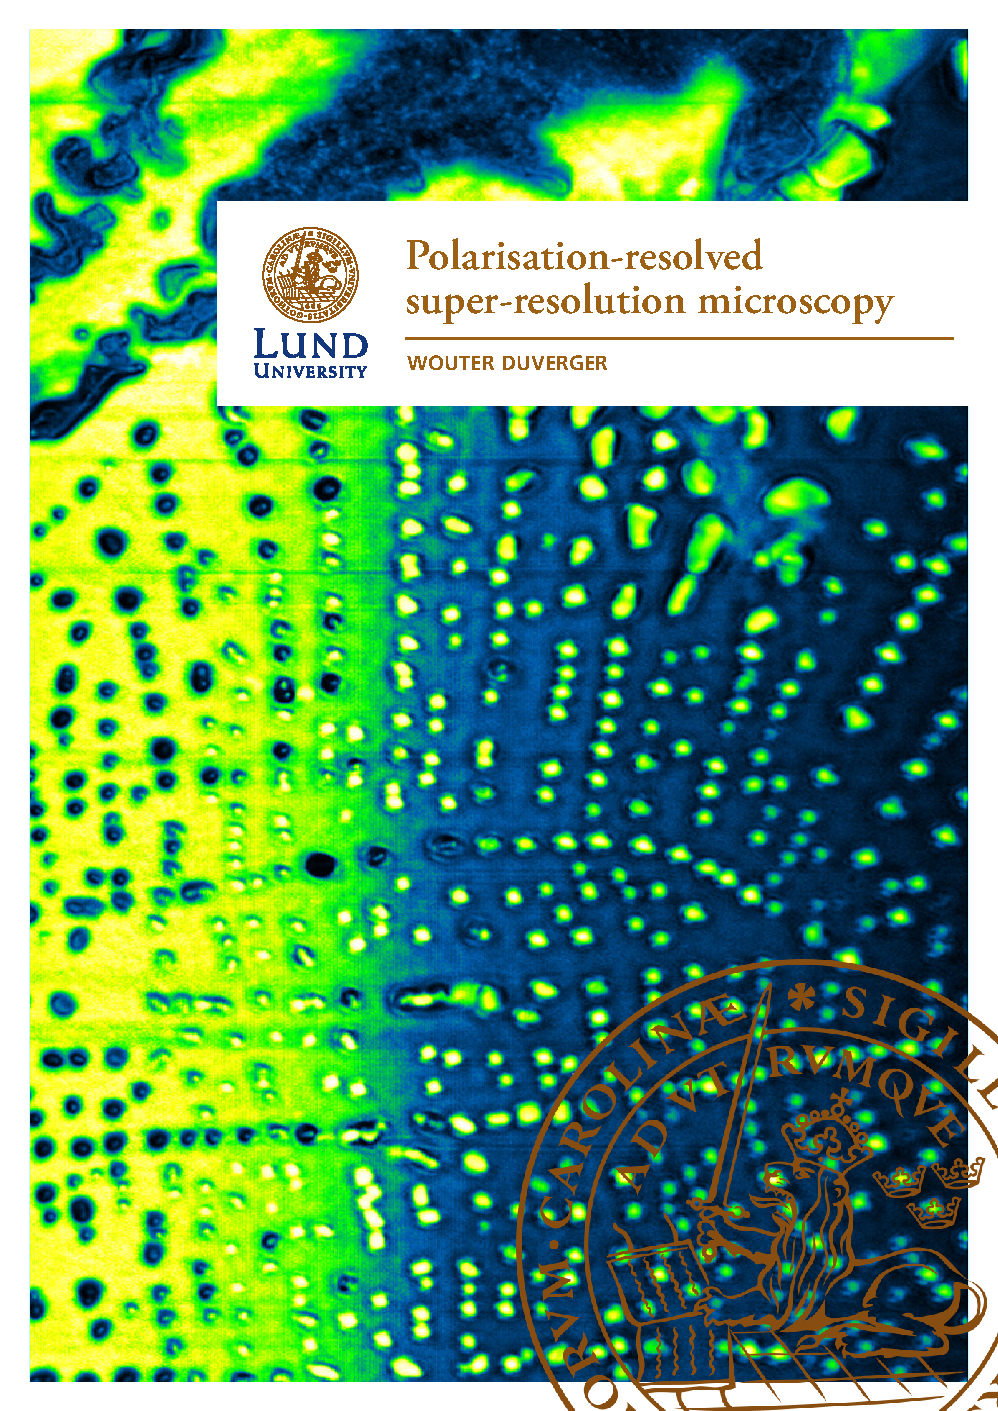
\includegraphics[page=1]{coverpage_g5.pdf}};
\end{tikzpicture}

\clearpage

\begin{titlepage}
	
	\frutigerfont
	
	\begin{center}

		
		{\Huge \garamondfont \thetitle}
		
		\smallskip
		by
		\bigskip
		
		{\Large \garamondfont \theauthor}
		
		\bigskip
		\bigskip
		
		This thesis is conducted in partial fulfilment of the requirements for the degree of 
		
		\bigskip
		
		{MSc in Physics} \\
		Biological Physics and Computational Biology,
		
		\bigskip
		
		at the NanoLund Centre for Nanoscience, Lund University,\\
		to be defended publicly on \todo{May ??, 2021}.
		
		
		\vspace{5cm}
		
		\vfill
		\begin{tabular}{ll}
			Project duration & 4 months (full-time equivalent)\\
			Supervision & Prof. Dr. Jonas Tegenfeldt\\
			Daily supervision & Dr. Jason Beech\\
			Examiner & Prof. Dr. Edouard Berrocal
		\end{tabular}
	
		\bigskip
	
		Cover image: artifacts of an old actin-phalloidin stained sample.
	
		\vspace{2cm}
		
		
\includegraphics[width=0.5\linewidth]{nanolund_logotype.pdf}
	
	
	\end{center}
\end{titlepage}

%\cleardoublepage
%
%{
%\raggedleft
%
%\vspace*{\fill}
%
%
%``Space separates bodies, not minds.''\\
%-- Erasmus of Rotterdam
%
%\vspace*{\fill}
%
%
%}
%
%\cleardoublepage

}
	
\frontmatter

	% !TeX spellcheck = en_GB
\chapter{Abstract}

This project aims to implement polarisation microscopy on the Tegenfeldt STED (stimulated emission depletion) microscope. STED microscopy is a targeted optical super-resolution method that can attain sub-diffraction resolution using visible light. This is now complemented with polarisation microscopy, which can measure the orientation of a fluorophore and, by extension, the molecule it is bound to. The current setup is one of the first systems in the world to combine STED and polarisation, but the its polarisation microscopy capability has never been tested.

In this thesis, I have characterised the effect of the various optical components in the microscope on the polarisation state of light and how they should be calibrated to perform several variations of polarisation microscopy. In the process, we have also developed a method that applies the operating principle of STED to increase resolution in the polarisation domain, which we call pSTED (polarisation-resolved stimulated emission depletion). The preliminary results are promising, but more work is required to demonstrate its potential as a new and innovative microscopy method.

All of the above methods have been applied to biological samples of human cell lines in which the actin cytoskeleton was fluorescently stained. The cells in these samples have been exposed to Yersinia bacteria. Pathogenic members of the Yersinia genus, of which the plague-causing \emph{Y.~pestis} is a member, destroy the actin cytoskeleton. In the absence of large actin fibres, it has been found that actin can form self-organising patterns on the microscale. This discovery opened up an exciting line of research where polarisation microscopy will be highly applicable.
	
	\renewcommand{\contentsname}{Table of Contents}
	\tableofcontents
	\addcontentsline{toc}{chapter}{Table of Contents}	
	
	% !TeX spellcheck = en_GB
\chapter{Nomenclature}

\begin{tabular}{ll}
	APD   & Avalanche photodetector                                                              \\
	AOM   & Acousto-optical modulator                             \\
	CCD & Charge-coupled device                               \\
	GFP   & Green fluorescent protein                                                            \\
	HWP   & Half-wave plate                                                                      \\
	MPE   & Maximum permissible exposure                             \\
	NA & Numerical aperture                            \\
	OD    & Optical density  (an OD2 filter reduces the light intensity by a factor of $ 10^2 $) \\
	PMT   & Photomultiplier tube                                                                 \\
	PSF   & Point spread function                                                                \\
	pSTED & Polarisation-resolved stimulated emission depletion microscopy                       \\
	QWP   & Quarter-wave plate                                                                   \\
	SiR   & Silicon-rhodamine                                                                    \\
	SLM   & Spatial light modulator                                                              \\
	STED  & Stimulated emission depletion  microscopy                                            \\
	TCSPC & Time-correlated single photon counter
\end{tabular}

\mainmatter

	% !TeX spellcheck = en_GB
\chapter{Introduction}
Between 1900 and 2000, advances in public health have increased life expectancy by 25 years \cite{Bunker1994}. The Centers for Disease Control and Prevention (CDC) credits advances in molecular biology such as vaccinations, better prevention of infectious diseases, better treatment of coronary heart disease and stroke, and more \cite{CDC1999}. Another pillar of molecular biology is the rapid development of SARS-CoV2 vaccines in the current pandemic \cite{Sadoff2021, Polack2020}. There are still many incurable diseases in the world, but by studying how they work, we can learn how cells and organisms function, and propose new treatments. Studying one disease can also guide treatment of another, as was the case when research into amyloidoses (a group of diseases including Alzheimer's disease, Parkinson's disease and diabetes type II, characterised by toxic amyloid protein aggregation), spun off a new direction of research into cancer treatment \cite{Gallardo2016}.

This thesis is part of a research programme that studies Yersinia. Yersinia is a genus of bacteria that includes \emph{Y. pestis}, which causes the plague, estimated to have killed millions of people in the Byzantine empire in the 6\textsuperscript{th} century CE, and again 50 million in Europe in the 14\textsuperscript{th} century, which was at that point about one third of the entire population \cite{Zietz2004}. Vaccinations are now available and the incidence is low, at less than 1000 cases per year worldwide \cite{WHO2014}. 
While there is no direct clinical need for more research into Yersinia, it is still a fascinating subject of fundamental importance, since it has an interesting mode of action. Yersinia bacteria secrete toxins into the cell that break down the actin network \cite{Ono2017}. The actin cytoskeleton works like the bones and muscles of a cell and is therefore vital to all kinds of processes, including embryonic development, cancer metastasis, and the immune system \cite{molbio, Horwitz2003, Umeda2016, Barnat2017, Lin2017}. Furthermore, it has been discovered that the absence of large actin fibres reveals self-organising actin microstructures \cite{Fritzsche2017a}. Their presence was quite a surprise and studying them may lead to new fundamental discoveries about actin and its role in healthy cell function.

The goal of this thesis is to set up a polarisation-resolved super-resolution fluorescence microscope to study these actin microstructures.	Microscopy -- imaging structures at microscopic scales -- is a wide and varied field. Microscopy was born in the sixteen hundreds, with Antoni van Leeuwenhoek's discovery of bacteria and other single-celled organisms \cite{VanZuylen1981}. Over time, the resolution of microscopes has strongly improved, and as lenses got better and better, they stopped being the resolution bottleneck. In 1873, Ernst Abbe determined that the best possible focus that a microscope can reach is limited by the wavelength of the light used \cite{Abbe1873}. This meant that microscopes of the time were limited to a resolution of roughly 200~nm (assuming focused blue light). It was long believed that the Abbe limit was a fundamental limit of nature, and that the only way around it was to use light of a different wavelength. This is one of the reasons for the development of electron microscopes, as quantum mechanics explains that accelerated electrons have a much shorter wavelength than visible light \cite{Smith2008}. 

However, using visible light for microscopy has some major advantages that electron microscopy cannot provide. Unlike with other methods, it is possible to tag specific protein species and other relevant molecules in the cell with a fluorescent label. For that reason, fluorescence microscopy has been an invaluable tool in modern biology \cite{Danial2016}.  There are thousands of small organic fluorescent labels available, and more are still being developed \cite{Zhang2002, Resch-Genger2008}. The introduction of GFP and other fluorescent proteins was a remarkable development in the field, as labels can now be genetically fused to proteins of interest \cite{Shaner2005, Matlashov2020}. In the year 2020 alone, over twenty thousand papers indexed in the PubMed database mention fluorescence in their title or abstract.

Fluorescence microscopy is not only capable of reporting on the location of a fluorophore, but also on its orientation. This is because fluorophores have a transition dipole moment; they will not absorb light that is polarised perpendicular to that dipole, and will only emit radiation polarised parallel to it. Therefore, fluorescence emission anisotropy is related to the dipole moment, which is determined by the orientation of the molecule that the fluorophore is bound to.

The group in which I conducted this thesis project, led by Jonas Tegenfeldt, already owned a stimulated emission depletion (STED) microscope, capable of performing fluorescence microscopy below the Abbe limit. It was fitted with some extra optics to enable polarisation microscopy by the supplier (Abberior GmbH, Germany), but as they had never done STED and polarisation microscopy at the same time, these capabilities were untested at the start of my thesis project. Therefore, the main goal of this thesis was to test the setup and properly calibrate it for polarisation microscopy experiments. Most of my learnings and contributions will hence be found in the Background and Methods sections of this report. Along the way, we also came up with the idea of applying the working principle of STED in the polarisation domain and invented a microscopy protocol we call polarisation-resolved stimulated emission depletion microscopy (pSTED), which will be discussed in the Methods section.
	% !TeX spellcheck = en_GB
\chapter{Background}

This section introduces concepts and techniques essential to this thesis. First, I will explain how fluorescence arises from discrete molecular energy states. Then, I will explain how the wave nature of light limits the resolution of a microscope by limiting the size of the focal spot to roughly half the wavelength of the light used, and two methods to get around it. The first method, STED microscopy, uses targeted quenching of fluorescent molecules (also called dyes or fluorophores) at the edge of the focal spot to effectively narrow down the spot size. The second method exploits the polarisation state of excitation or emission light to measure the orientation of certain structures in a sample, even if their size is below the resolution limit.

\section{Fluorescence microscopy}

In short, fluorescence is a phenomenon in which a molecule absorbs a photon of one wavelength, spends a short amount of time (a couple of nanoseconds) in an excited energy state, and then emits a photon of a wavelength longer than the first one. The difference in wavelength, called the Stokes shift, is essential to perform microscopy, and the fact that molecules have discrete energy states is key  to generate that difference.

\begin{figure}
	\centering
	 \includegraphics[height=.4\linewidth]{jablonski diagram.ai} \hfill 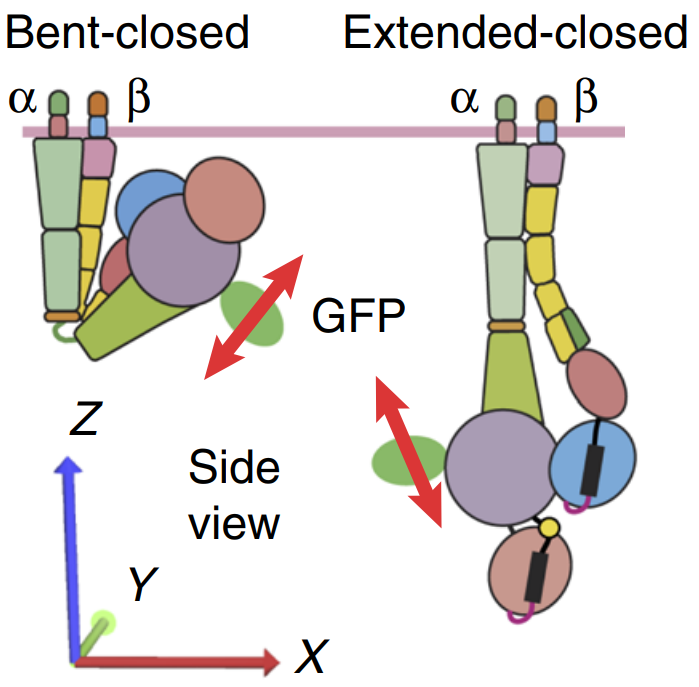
\includegraphics[height=.4\linewidth]{nordenfelt et al.png}
	\caption{
		\textbf{Left:} Illustration of the discrete energy states of a molecule and some possible transitions between them. The difference between energy levels determines the wavelength and colour of the absorbed or emitted photon. $ S_1 $ and $ S_2 $ are electronic energy levels that each contain a set of vibrational states. \textbf{Right:} Illustration of how a fluorophore's dipole moment (red arrow) can report on the orientation of the molecule it is bound to. In this case, the fluorophore is GFP (green fluorescent protein) and the target is a transmembrane integrin protein with subunits $ \alpha $ and $ \beta $. Image by Nordenfelt et al.~\cite{Nordenfelt2017}.
	}
	\label{fig:jablonski}
\end{figure}

Let us consider a molecule with two electronic energy states, each of which has a number of vibrational energy levels as in \autoref{fig:jablonski}. When the molecule is in its ground state (the lowest available energy level, $ S_0 $), it can absorb photons only if the energy they carry matches the difference between the ground state and another energy level. From an excited state ($ S_1 $), the system can relax into lower vibrational levels without emitting radiation, after which it emits a photon and relaxes back to the ground state. Two possible paths are shown in the figure. Because some energy is lost in a non-radiative way, the emitted photons will carry less energy than the absorbed photon, resulting in the wavelength difference mentioned before. This is called the Stokes shift. 

We can make that a little more rigorous by considering what happens to a simplified two-level quantum system such as a hydrogen atom subject to a Hamiltonian $ H_0 $. Denote the energy states of the electron with $ \ket{1} $ and $ \ket{2} $. These are eigenstates of the Hamiltonian with energy $ \epsilon_i $. When exposed to an electric field $ \vb{E} = \vb{E}_0 \cos\omega t$, the Hamiltonian is perturbed: $ H' = H_0 + \vb*{\mu} \cdot \vb{E}(t) $, where $ \vb*{\mu} = -e\vb{r}$. If the system is in the ground state at time $ t=0 $, the probability to find it in the excited state at time $ t $ is given by
\begin{equation}
	\abs{c_2(t)}^2 = \abs{\mel{2}{e^{-iHt/\hbar}}{1}}^2.
\end{equation}
For weak fields, a first-order approximation is
\begin{equation}
	\abs{c_2(t)}^2 = \abs{ \frac{\vb*{\mu}_{21}\cdot\vb{E}_0}{\hbar}  \frac{\sin((\omega_0-\omega)t/2)}{\omega_0-\omega}}^2,
	\label{eq:transition moment}
\end{equation}
where $ \vb*{\mu}_{21} = \mel{2}{\vb*{\mu}}{1} $ and $ \omega_0 = (\epsilon_2-\epsilon_1)/\hbar $. More detail can be found in C.J.~Foot \cite{Foot}. From this equation, we can conclude that there are two conditions for a transition. Firstly, the frequency of the electric field $ \omega $ must match the energy difference between the states $ \omega_0 $. (Note that we have not made any statement about the sign of $ \omega_0 $. This process can represent absorption as well as stimulated emission.) Secondly, the electric field is most effective at driving the transition when it is polarised along the transition dipole moment $ \vb*{\mu}_{21} $. For example, if an electron is confined to a chemical bond, it will not interact with electric fields polarised orthogonal to that bond. The precise energy levels available depend on the molecule and its environment. Therefore, every fluorescent molecule has a unique absorption and emission spectrum, which needs to be considered when planning a fluorescence experiment.

\section{The diffraction limit}

The resolution of fluorescence microscopy used to be limited by light diffraction. Consider the diffraction limit in one of the simplest possible setups: an epifluorescence microscope. Epifluorescence microscopy is fairly similar to bright field microscopy; it just uses excitation light of a well-defined wavelength instead of white light. The sample, which is stained with a fluorescent dye, is illuminated at a wavelength that dye can absorb. The dye molecules will then emit photons of longer wavelengths in their emission spectrum, which are collected by the microscope objective. Before imaging by a CCD camera, scattered laser light can be filtered away using a dichroic mirror that passes emission light and reflects excitation light. 


It used to be the case that microscopes were limited in resolution by the quality of their lenses and the pixel density of the CCD, but there is a much more fundamental limit, first described by Ernst Abbe. This limit is caused by the presence of an aperture. When a beam of light goes through an aperture of finite size, such as a lens, it cannot be focused onto an infinitesimally small point. Instead, it will generate a spot with a radius approximately equal to $ \lambda/2\na $, where $ \lambda $ is the wavelength of the light and $ \na= n\sin\theta $ is the numerical aperture, the product of the index of refraction and the sine of the half-cone angle of the acceptance cone.

\begin{figure}[!t]
	\centering
	\begin{tabularx}{\linewidth}{lXl}
		\toprule
		& Criterion                                                                            & Definition                            \\ \midrule
		Rayleigh & The first minimum of one point's Airy function coincides with the maximum of another & $ d_{xy} = .61\lambda/\na $           \\
		FWHM     & The width of the Airy function at half of the peak height                            & $ d_{xy} = .51\lambda/\na $           \\
		Abbe     & Resolving all groups of the 19-group Nobert plate \cite{Abbe1873, Norbert}                                  & $ d_{xy} = \phantom{1}.5\lambda/\na $ \\
		Sparrow  & The distance between fluorophores at which the central maximum splits                & $ d_{xy} = .47 \lambda/\na $          \\ \bottomrule
	\end{tabularx}
	\captionof{table}{Some common definitions of the resolution limit $ d_{xy} $.}
	\label{tab:resolution limits}
	
	\centering
	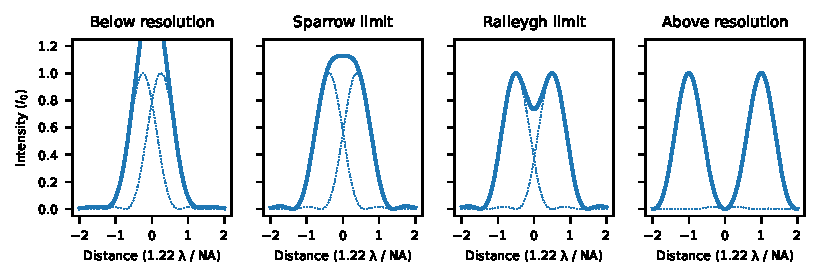
\includegraphics{diffraction_limit.pdf}
	\captionof{figure}{
		Illustration of the diffraction limit. Below the resolution limit, two fluorophores (with PSF dashed) appear under a microscope as a single peak (solid, sum of the intensities of the two fluorophores). Distance is measured in multiples of the Rayleigh limit ($ .61\lambda/\na $).
	}
	\label{fig:diffraction limit}
\end{figure}

In particular, a circular aperture will convert point sources in the sample plane to Airy patterns in the image plane. Mathematically, this can be described by a convolution product between the point spread function (PSF) $ h_\mathit{det} $ and the fluorophore distribution $ \rho $,
\begin{equation}
	I(\vb{x}) = (h_\mathit{det} * \rho)(\vb{x}) \coloneqq \int\dd{\vb{x}'} h_\mathit{det}(\vb{x}-\vb{x}')\rho(\vb{x}'),
	\label{eq:convolution}
\end{equation}
where the triple integration over the three components of $ \vb{x}' $ is implied, resulting in an image $ I(\vb{x}) $. When two fluorophores are close enough together that their PSFs overlap, they appear as a single object instead of two separate ones. This happens when the distance between them is around $ \lambda/2\na $, and that is what determines the resolution of a microscope. The exact resolution depends on your definition of this minimum resolvable distance. There are several definitions, but they are all proportional to $ \lambda/\na $. Some of them are listed in \autoref{tab:resolution limits} and visualised in \autoref{fig:diffraction limit}.



For a long time, physicists thought this limit was practically unavoidable \cite{McCutchen1967}, but in the next sections, I will discuss two ways in which one can get information from a system below the resolution limit. The first method (STED microscopy) directly increases the image resolution. The excitation light is still subject to the Abbe limit, but we add another laser to effectively improve our focusing. The second is indirect and requires playing with a new aspect of light (polarisation) that allows you to get orientational information about structures that are otherwise below the resolution limit.

\section{Super-resolution microscopy}

\begin{figure}
	\centering
	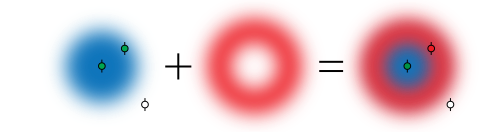
\includegraphics[width=\linewidth]{sted.ai}
	\caption{
		Working principle of STED microscopy. Fluorophores at the edge of the excitation PSF are quenched by stimulated emission, effectively resulting in a narrower PSF. Both beams are circularly polarised. 
	}
	\label{fig:sted principle}
\end{figure}

There are several ways to increase image resolution directly, many of which use the photophysics of individual dyes to turn off a subset of them during imaging. Some methods do this stochastically, such as STORM (stochastic optical reconstruction microscopy) and PALM (photoactivated localisation microscopy) \cite{Mock2009, Betzig2006}. These localisation-based methods activate a random subset of fluorophores, such that the average distance between them is above the resolution limit. Then they are imaged with a camera and the centres of their PSFs are estimated. The precision of that estimate scales with $ 1/\sqrt{N} $ where $ N $ is the numbers of photons collected.

On the other hand, there are targeted techniques such as STED (stimulated emission depletion), GSD (ground state depletion), RESOLFT (Reversible saturable optical fluorescence transitions), and more \cite{Klar2000, Folling2008, Hofmann2005}. Generally, they work by turning off fluorophores on the outer edge of the focal spot (depletion). The resolution achieved is dependent on the intensity of the depletion laser. This is a case of targeted instead of stochastic photoswitching. The Tegenfeldt group own a STED microscope, so that is what I will focus on in this section. 

In essence, a STED microscope is a scanning confocal microscope with an extra laser that can selectively deplete fluorescence by stimulated emission. Its working principle is shown in Figures \ref{fig:sted principle} and \ref{fig:sted microscope}. In a scanning confocal microscope, the excitation laser does not illuminate the whole sample at once, but is scanned over it. This means only fluorophores in an Airy disk around the focus will be excited. Furthermore, the detector is now comprised of a pinhole and a photodetector (not a camera), which filters out most of the out-of-focus light \cite{Minsky1957}. Therefore, the PSF of a confocal microscope is the product of the laser PSF $ h_\exc $ and the detection probability $ h_\mathit{det} $
\begin{equation}
	h_\mathit{conf}(\vb{x}) = h_\exc(\vb{x}) \cdot h_\mathit{det}(\vb{x}),
\end{equation}
where the most important characteristic of $ h_\mathit{det}(\vb{x}) $ is that it is quite narrow in the $ z $ direction. The smaller the detection pinhole, the stronger this effect. However, a smaller detection pinhole also means that even a fraction of the light from the focal plane will be rejected from the photodetector. Therefore, there is a trade-off between $ z $ resolution and the signal-to-noise ratio (SNR).

Even though both of these PSFs are diffraction-limited, a STED microscope can reach an arbitrarily small resolution \cite{Wildanger2012}. It does so by illuminating the sample with a donut-shaped laser at a wavelength longer than the emission wavelength. Referring back to \autoref{fig:jablonski}, the blue laser excites the fluorophores that emit in green, but a red transition is also allowed. Under illumination with a red laser, this transition is made more favourable by the process of stimulated emission, first postulated by Einstein in 1926 \cite{Einstein1926}. This way, fluorophores at the edge of the excitation PSF can be prevented from emitting green light, while fluorophores at the centre do not experience stimulated emission, which reduces the width of the effective point spread function. An illustration of this effect is given in \autoref{fig:sted principle}.


Mathematically, the STED beam depletes fluorescence according to
\begin{equation}
	\eta(\vb{x}) = \exp(-\sigma_\dep h_\dep(\vb{x})),
\end{equation}
which relates the fraction of fluorescence remaining as a function of the depletion intensity $ h_\dep $. Therefore, the STED point spread function can be expressed as
\begin{equation}
	h_\mathit{STED} = h_\exc(\vb{x}) \cdot \eta(\vb{x}) \cdot h_\mathit{det}(\vb{x}),
\end{equation}
which can be read as ``the probability for a dye to be excited, times the probability for it not to be quenched by stimulated emission, times the probability for fluorescence emission to be detected by the CCD''. Even though every individual PSF ($ h_\exc(\vb{x}) $, $ h_\dep(\vb{x}) $ and $ h_\mathit{det}(\vb{x}) $) is diffraction-limited, the fact that you need to multiply them results in a narrowing of the effective PSF below the Abbe limit. This means that the extent of the resolution improvement depends on the intensity of the depletion laser $ I_\dep$. Harke et al.~approximate the STED resolution as
\begin{equation}
	d_\mathit{STED} = \frac{d_c}{\sqrt{1+d_c^2a^2\cfrac{I_\dep}{I_\mathit{sat}}}},
\end{equation}
where $ d_c $ is the resolution limit of a confocal microscope, $ a $ the steepness of the donut pattern (i.e.~high $ a $ means very tight central minimum in the donut-shaped intensity), and $ I_\mathit{sat} $ is the depletion intensity at which fluorophore brightness is reduced by half \cite{Harke2008}.

\begin{figure}
	\centering
	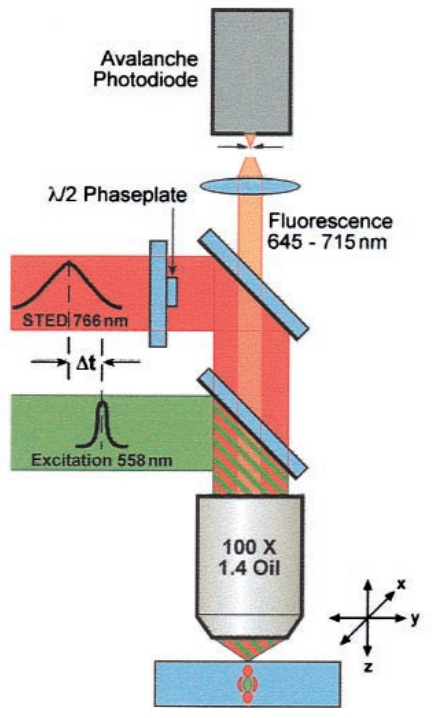
\includegraphics[width=0.3\linewidth]{sted microscope schematic.png}
	\caption{
		The rough layout of a STED microscope. The excitation laser is focused on the sample, and the STED laser forms a donut pattern around the focal spot. Emitted light is collected by the objective and focused on a pinhole before it is detected by an APD. Figure from Klar et al.~2000 \cite{Klar2000}.
	}
	\label{fig:sted microscope}
\end{figure}

Although STED can reach an arbitrary resolution under optimal circumstances, the resolution reached in biological specimens is more usually around 50~nm \cite{Wildanger2012,Muller2012}. If information is desired at an even smaller scale using fluorescence microscopy, then other methods are required.
There are several reasons the resolution of STED in biological samples has not been able to reach the single-nanometre scale. One is that these samples consist of cells in a water-based solution, which causes a strong mismatch in the index of refraction between the sample and the optics used (commonly glass and oil). Another is the limited photostability of the dyes. Every time a fluorophore absorbs a photon, there is a probability that a photochemical event occurs that damages (bleaches) the fluorophore. Good fluorophores can typically absorb 10 000 to 40 000 photons before this happens \cite{Lichtman2005}. Therefore, high excitation powers result in high bleaching rates. Photobleaching is mainly due to interactions with reactive oxygen species and is therefore not only determined by the properties of the fluorophore, but also the environment. Photobleaching can also be induced by other causes, such as the absorption of multiple photons. Refer to Diaspro et al.~for an overview of photobleaching \cite{Diaspro2006}. When imaging live cells, phototoxicity also needs to be taken into account. Because molecules other than the targeted fluorophores can also absorb laser light (possibly resulting in autofluorescence), incident radiation can be toxic for the cell, for the same reasons as it can bleach a fluorophore \cite{Lichtman2005}. Therefore, photobleaching and phototoxicity both limit the laser power that can be applied.


\section{Polarisation microscopy}

Polarisation microscopy uses the vectorial nature of light -- the fact that light consists of electromagnetic waves that with a certain polarisation -- to get orientational information of fluorophores below the resolution limit. Other methods to get information on distances below the resolution limit  include fluorescence resonance energy transfer (FRET), for example, which is great for measuring distances between two fluorophores on the order of nanometres \cite{Lerner2021}.

Among others, light polarisation microscopy has been used to measure how the structure of DNA changes when it is subject to a strong stretching force, how integrin proteins respond to an applied force and the order of molecules embedded in the cell membrane \cite{Backer2019, Nordenfelt2017, Swaminathan2017, Brasselet2013}. In this section, I will first introduce the concept of light polarisation, then discuss how it can be used in a microscope, and finally mention some optical components that affect the light polarisation, which are crucial to conducting a polarisation microscopy experiment. For a more exhaustive introduction to polarisation microscopy, there are several good resources available \cite{Goldstein2011, Collett2005, Lakowicz2006}.

\subsection{The polarisation ellipse.} Light is a transverse electromagnetic wave, meaning that there are oscillations of the electric and magnetic field along the path of a light ray, and that these oscillations are orthogonal to the propagation direction. In other words, if the light propagates along $\vb{k}$, the electric and magnetic fields $\vb{E}$ and $\vb{B}$ must satisfy $ \vb{E} \cdot \vb{k} = \vb{B} \cdot \vb{k} = 0$. (The fields themselves are also orthogonal to each other, so we can neglect $ \vb{B} $ without compromising our analysis.)

For the sake of simplicity, let us consider a ray propagating in the $ z $ direction. The electric field at any point in space and time can be written as
\begin{align}
	E_x(z, t) &= \Eox \cos(kz-\omega t + \phi_x),\\
	E_y(z, t) &= \Eoy \cos(kz-\omega t + \phi_y).
\end{align}
where $ \vb{E}_0 $ is the amplitude of the oscillation, $ k $ is the wavenumber (the length of $ \vb{k} $), $ \omega $ is the radial frequency and $ \phi $ is an arbitrary phase. Note that the wavenumber and the frequency are related to each other through the speed of light $ c $, since $ \omega = kc = \hbar c/\lambda$. Note also that the $ x $ and $ y $ components can have a phase difference.

Letting $ \delta = \phi_y-\phi_x $, it can be shown that 
\begin{equation}
	\left(\frac{E_x}{\Eox}\right)^2 - 2\cos\delta\frac{E_x}{\Eox}\frac{E_y}{\Eoy} + \left(\frac{E_y}{\Eoy}\right)^2 = \sin^2\delta,
\end{equation}
which is the equation for an ellipse. This means that at any point in time, the point $ (E_x, E_y) $ lies on the ellipse defined by the equation above, which is called the polarisation ellipse and is completely determined by $ \Eox $, $ \Eoy $ and $ \delta $. Together, these values determine whether the polarisation is linear, circular, or something in between. Refer to \autoref{tab:polarisation states} for an overview.

\begin{table}
	\centering
	\begin{tabular}{lcccc}
		\toprule
		Polarisation state      & $ \Eox $ & $ \Eoy $ & $ \delta $ &     Jones vector      \\ \midrule
		Linear along $ x $      &    1     &    0     &    any     & $ (1, \phantom{-}0) $ \\
		Linear along $ y $      &    0     &    1     &    any     & $ (0, \phantom{-}1) $ \\
		Linear at \ang{+-45}    &    1     & $ \pm1 $ &     0      &     $ (1, \pm1) $     \\
		Circular (right-handed) &    1     &    1     & $ \pi/4 $  & $ (1, \phantom{-}i) $ \\
		Circular (left-handed)  &    1     &    1     & $ -\pi/4 $ &      $ (1, -i) $      \\ \bottomrule
	\end{tabular}
	\caption{List of a number of polarisation states (not normalised).}
	\label{tab:polarisation states}
\end{table}


In general, the polarisation ellipse can be defined by means of two angles: the orientation $ \psi $ and ellipticity $ \chi $, as shown in \autoref{fig:pol ellipse}. They can be calculated from $ \alpha = \arctan(\Eoy/\Eox) $ and the phase difference $ \delta $ using
\begin{align}
	\tan 2\psi &= \tan 2\alpha \cos \delta,\\
	\sin 2\chi &= \sin 2\alpha \sin \delta
\end{align}
This definition of $ \chi $ is dependent on the ratio of the maximum and minimum amplitude of the electric field as is presented in \autoref{fig:pol ellipse}. One can define a similar value based on the corresponding intensities. Since $ I = \abs{\vb{E}_0}^2 $,
\begin{align}
	\chi_I &= \arctan {I_\mathit{max}}/{I_\mathit{min}} = \arctan\left[ \left( {E_\mathit{max}}/{E_\mathit{min}} \right)^2 \right] .
\end{align}
To distinguish between them, I will be using $ \chi_E $ and $ \chi_I $ from now on. These are useful concepts because they are relatively easy to calculate from intensity measurements. Therefore, I will use them when I characterise laser beams in the setup.

\begin{figure}
	\centering
	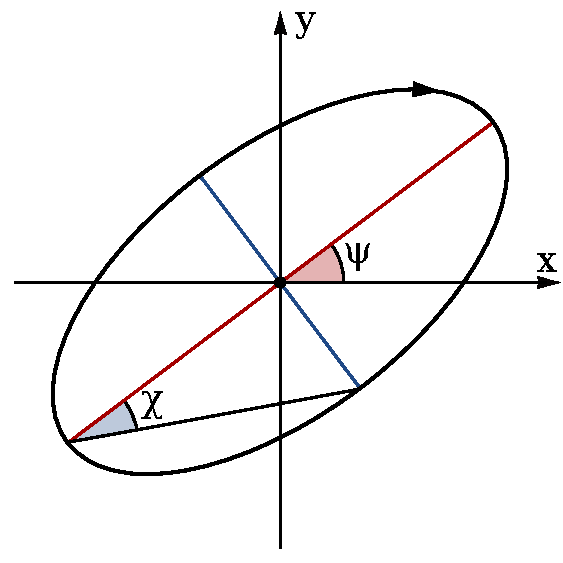
\includegraphics[width=.3\linewidth]{polarisation_ellipse.pdf}
	\caption{The meaning of $ \psi $ and $ \chi $ in the context of the polarisation ellipse. (Figure by Wikipedia user Inductiveload)}
	\label{fig:pol ellipse}
\end{figure}

\subsection{Microscopy.} Why is polarisation relevant to microscopy? Well, the probability of excitation is dependent on the polarisation of incoming light. Since a fluorophore can be considered a small dipole moment, it will not interact with radiation that is orthogonal to the transition dipole moment of the fluorophore (see discussion surrounding \autoref{eq:transition moment}). If the excitation laser is polarised along an angle $ \psi $ and the dipole is oriented along $ \theta $, the intensity of light emitted by that fluorophore will satisfy 
\begin{equation}
	\label{eq:malus}
	I(\psi, \theta) \propto \cos^2(\psi-\theta).
\end{equation}
This is Malus's law. Analogously, light emitted from a fluorophore is always linearly polarised parallel to the transition dipole moment. One can place a linearly polarising filter in front of the detector to measure a fluorophore's orientation. If the polariser emits light polarised at an angle $ \psi $, then the intensity measured at the detector also follows Malus's law, meaning that these two setups are analogous (not taking into account depolarisation effects in an experimental setup). As an example, see \autoref{fig:composite}. Dipole excitation by circularly polarised light is usually not dependent on $ \theta $, but there are fluorophores that are sensitive to the handedness of circularly polarised light \cite{Takaishi2019}.

Common polarisation microscopy protocols include: rotating a linearly polarised excitation laser, rotating a polarising filter in the excitation beam path, or doing both. The first polarisation measurements were done by excitation of the sample with a linearly polarised laser and measuring the fractions of emission intensity that were parallel and orthogonal to the excitation light. With those, one can calculate the anisotropy of a sample \cite{Camacho2019}. I will elaborate on different polarisation microscopy methods in \autoref{sec:pol analysis}. 

\subsection{Jones calculus.} Lasers are usually linearly polarised, but I have not yet mentioned how we can manipulate this polarisation to run the experiments we want. There are optical elements such as waveplates that can do this for us, and the best way to understand them is through Jones calculus. This is an incredibly useful way to model light polarisation, but it does require us to express the electric field as a complex function:
\begin{equation}
	\vb{E}(z, t) = \vb{E}_0 e^{i(kz-\omega t)}.
	\label{eq:propagator}
\end{equation}
In the following analysis, we will treat $ \vb{E} $ as a two-dimensional vector with only an $ x $ and $ y $ component, since $ E_z = 0 $. Note that complex numbers are just a mathematical trick. The Maxwell equations that govern light propagation are linear, and taking the real part of a complex-valued function is also a linear operation, so the complex extension of $ \vb{E} $ will behave exactly like the actual electric field would. The phase difference between the two components is now contained in $ \vb{E}_0 $, which can be expressed as
\begin{equation}
	\vb{E}_0 = \mqty(\Eox \\ \Eoy e^{i\delta} ).
\end{equation}
Therefore, $ \vb{E}_0 $, the Jones vector, contains all information about the polarisation state of a beam. The Jones vectors for some special polarisation states are listed in \autoref{tab:polarisation states}.

The usefulness of Jones calculus lies in its ability to represent optical components as matrices acting on this vector. For example, a polariser that transmits $ x $-polarised light has the following matrix form:
\begin{equation}
	S_p = \mqty(1 & 0 \\ 0 & 0).
\end{equation}
It is easy to verify that $ S_p \vb{E}_0 = \Eox $. 

We also need to take into account how mirrors affect polarisation. In this case, it is useful to define a new coordinate system. Let $ k $ be the propagation direction, $ p $ the direction that is orthogonal to $ k $, but in the plane of incidence (the plane formed by $ k $ and the normal to the mirror surface, i.e. $ p $ is parallel to the plane of incidence). Finally, let $ s $ be orthogonal to $ k $ and $ p $ ($ s $ stands for the German word senkrecht). Mirrors flip the $ s $ component of the field polarisation, while keeping $ p $ unchanged. So, a mirror whose surface is parallel to the $ x $-axis has a Jones matrix of the form
\begin{equation}
	S_{mx} = \mqty(1 & 0 \\ 0 & -1).
\end{equation}

Another important type of optical component in our setup is a waveplate. Waveplates or phase retarders are made out of birefringent crystals such as quartz, in which the index of refraction a ray of light experiences is dependent on its polarisation. This happens when a crystal structure lacks cubic symmetry. When the coordinate system is aligned with the crystal axes, we might find that $ k_x = k_z = k_o $ (the ordinary axes), while $ k_y = k_e $ (the extraordinary axis). $ k_e $ may both be greater or less than $ k_o $. In these crystals, \autoref{eq:propagator} is no longer valid and should be replaced by
\begin{equation}
	\vb{E}(z, t) = \mqty(\Eox e^{i(k_o z-\omega t)} \\ \Eoy e^{i(k_e z-\omega t + \delta)} ).
\end{equation}
This can also be written in the form
\begin{equation}
	\vb{E}(z, t) = \mqty(\Eox  \\ \Eoy e^{i(\Gamma(z) + \delta)} ) e^{i(k_o z-\omega t)}
	\qq{, where}
	\Gamma(z) = (k_e-k_0) z.
\end{equation}
As one can see, a waveplate only imparts a delay on the $ y $-component of a beam, depending on its thickness $ z $ and its birefringence. We can neglect the phase factor common to both components and represent the action of a waveplate by the following Jones matrix in the local coordinate system of the waveplate with
\begin{equation}
	S_\Gamma = \mqty(1 & 0 \\ 0 & e^{i\Gamma}).
\end{equation}
We can name the axes in this coordinate system the fast and slow axes, where the field component along the slow axis incurs the phase delay.

Generally, waveplates are characterised by the relative delay they impart on polarisation components. Quarter-wave plates delay it by a quarter of a wavelength compared to the fast propagating ray, corresponding to $ \Gamma = (2n + 1/2)\pi $ (for any integer $ n $). Therefore, the Jones matrix of a quarter-wave plate satisfies 
\begin{equation}
	S_\qwp = \mqty(1 & 0 \\ 0 & e^{i\pi/2}) = \mqty(1 & 0 \\ 0 & i).
\end{equation}
Let's consider what happens to some specific cases. If $ x $ or $ y $ polarised light passes through a quarter-wave plate, its polarisation will not change. But light polarised along $ +\ang{45} $ ($ -\ang{45} $) will be turned into left-handed (right-handed) light, and vice versa. Therefore, a quarter-wave plate allows us to convert between linearly and circularly polarised light, as shown in \autoref{fig:waveplates}.

\begin{figure}
	\centering
	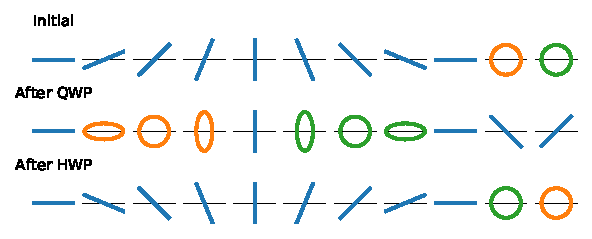
\includegraphics{waveplates.pdf}
	\caption{
		The effect of quarter-wave plates (QWP) and half-wave plates (HWP) on the polarisation ellipse. The fast axis is horizontal and indicated in the figure. The slow axis is vertical. Orange: left-handed polarisation. Green: right-handed polarisation. The ray is propagating into the page.
	}
	\label{fig:waveplates}
\end{figure}

The second type of waveplate we should treat is a half-wave plate. It features a delay of $ \Gamma = (2n+1)\pi $, and its Jones matrix looks like
\begin{equation}
	S_\hwp = \mqty(1 & 0 \\ 0 & e^{i\pi}) = \mqty(1 & 0 \\ 0 & -1),
\end{equation}
which corresponds to mirroring the polarisation state about the $ x $-axis. Another way to think about it is that a ray polarised along an angle $ \psi $ will be rotated by an angle $ -2\psi $, and the handedness of circularly polarised light will be reversed, see \autoref{fig:waveplates}.

The power of Jones calculus lies in its ability to model the behaviour of a sequence of optical elements at arbitrary rotations. First, we need to define the Jones matrix for a rotated component. This is simply
\begin{equation}
	S(\theta) = R(\theta) \cdot S \cdot R(-\theta),
	\qq{where} 
	R(\theta) = \mqty(\cos\theta & -\sin\theta \\ \sin\theta & \cos\theta)
\end{equation}
and $ \theta $ is the angle of the component's fast axis with the lab coordinate system's $ x $ axis. As an example, we can send $ x $ polarised light through a polarising filter at an angle $ \theta $, which results in
\begin{equation}
	I(\theta) \propto \abs{S_p(\theta) \cdot \mqty(1 \\ 0)}^2 = \cos^2\theta.
\end{equation}
That is Malus's law, as we had defined before. We can also recover the same behaviour by using a fixed polarising filter and a half-wave plate at an angle $ \theta/2 $:
\begin{equation}
	I(\theta) \propto \abs{S_p(0) \cdot S_\hwp(\theta/2) \cdot \mqty(\admat{1 \\ 0})}^2 = \cos^2\theta.
\end{equation}

Jones calculus has its limitations, the main one being that it cannot represent unpolarised light (an incoherent sum of different polarisations). Müller calculus, based on real-valued 4D Stokes vectors instead of the complex 2D Jones vectors, can handle it. As such, Müller calculus can also quantify depolarisation induced by non-ideal microscope optics. In this thesis, I mainly used Jones calculus to develop a theoretical understanding of the optical elements in the STED microscope, for which Müller matrices are not necessary. In the next sections, I will use the theory presented here to implement polarisation microscopy on the Tegenfeldt STED microscope. I will even develop the theory further to extend the concept of the optical point spread function into polarisation space.

	% !TeX spellcheck = en_GB
\chapter{Methods}

\todo{intro?}

\section{Microscope setup}

\begin{figure}[bh]
	\centering
	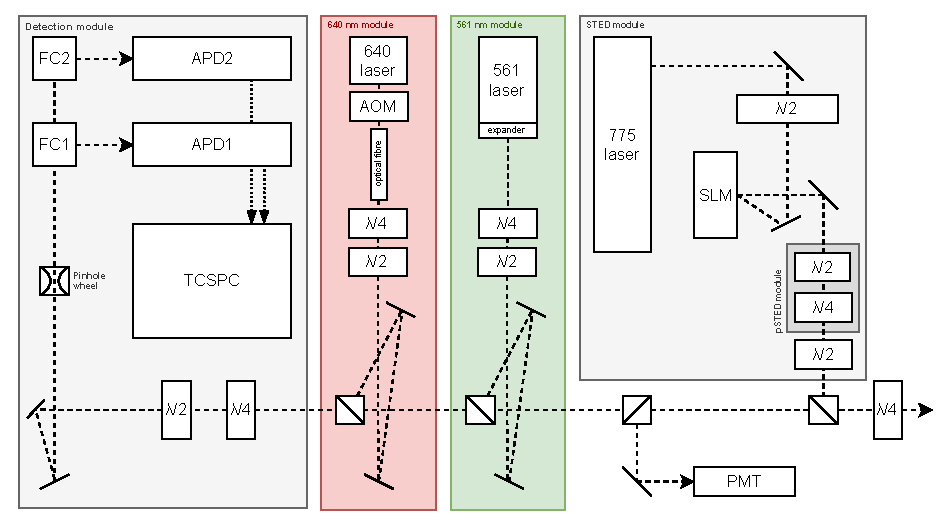
\includegraphics[width=\linewidth]{microscope layout.pdf}
	\caption{
		Schematic overview of the Tegenfeldt microscope. The sample is located in a microscope housing on the bottom right (outside this figure). FC1 and FC2 are swappable filter cubes. Half-wave and quarter-wave plates are denoted $ \lambda/2 $ and $ \lambda/4 $, respectively. Dashed lines represent the light path, except those that go to the TCSPC (those are digital connections). The waveplates in the pSTED module were not in the original setup, and were added as part of this project. See text for more details.
	}
	\label{fig:layout}
\end{figure}

In short, the Tegenfeldt microscope is a confocal fluorescence microscope constructed by Abberior Instruments GmbH (Germany). It features two excitation lasers (at 561~nm and 640~nm) and one depletion laser at 775~nm for two-channel confocal or STED microscopy. It also contains a time-correlated single photon counter (TCSPC) for fluorescence lifetime imaging microscopy (FLIM) and a highly sensitive photomultiplier tube (PMT). Refer to \autoref{fig:layout} for the layout of these optical elements. Samples are located inside an inverted Nikon microscope body (Ti-E, not shown in the figure) equipped with a piezo stage (M-687 PILine XY-stage system and P-736 PInano (Physik Instrumente) Z Microscope Scanner), a 60x, 1.4~NA oil immersion objective (Nikon Plan Apo) and a QUADScan beam scanner (Cambridge Technology).

In this section, I will address all laser lines as well as the detection module in detail, with a focus on characterising the light polarisation at different points in the microscope.

\paragraph{The laser modules.} The fast-switching 561~nm laser is initially horizontally polarised, but the polarisation can be tuned by three waveplates in its path. The last one, a quarter-wave plate, is fixed in its rotation angle. In the standard mode of operation, excitation laser light should be circularly polarised to minimise resolution reduction due to lens distortion etc. \cite{Harke2008}. In that mode, the (fast or slow) axis of the first quarter-wave plate should be aligned with the laser, such that it does not affect polarisation and the half-wave plate should be set such that it rotates the (linearly polarised) light to \ang{45} with respect to the second quarter-wave plate. See \autoref{tab:laser polarisation} for the polarisation characteristics in the calibration provided by Abberior. The 561~nm laser is quite well-calibrated. In circular polarisation, it reaches a $ \chi $ very close to perfectly circular (\ang{45}).

The 640 nm laser does not have fast-switching built in, so instead the light is fed into the microscope through a polarisation-polarisation optical fibre by an acousto-optical modulator (AOM). The AOM is a crystal in the beam path, in which sound waves can be generated by a piezo element. The ray is deflected by an angle that depends on the frequency of these waves, such that the laser beam can quickly be aligned into or away from the fibre aperture. The rest of the beam path is very similar to the 561 module, but the calibration of the waveplates in this pathway are not as accurate. Refer to \autoref{tab:laser polarisation}. 

The depletion laser travels through an entirely different set of optics than the excitation lasers to generate a donut beam. First, it travels through a half-wave plate that aligns the polarisation to the SLM (spatial light modulator). This HWP is necessary because an SLM adds an arbitrary spatially patterned phase delay to incident light, but only to the component polarised along its active axis. It will not alter the phase of the orthogonally polarised component. Using the proper phase delay patterns, one can create any (diffraction-limited) image in the sample plane. In our case, that would be a donut shape. Then -- and I am ignoring the pSTED module for now, since that was not included in the original setup -- the beam travels through a half-wave plate to ensure circular polarisation in the sample plane (after going through a quarter-wave plate at \ang{45} to the QWP axes), just like the excitation lasers. This is done to ensure that the depletion efficiency does not depend on sample orientation and to avoid polarisation-dependent PSF distortion by lenses and other optics. The quality of the STED polarisation is similar to that of the 640 nm laser. Note that this is actually a significant result, as that means the donut beam is not isotropically polarised. It will be far more effective at quenching fluorophores oriented at \ang{40} than those at \ang{130}.

\begin{table}
	\centering
	\caption{
		Polarisation characteristics of the lasers. Shown are linearity $ I_\mathit{max} / I_\mathit{min} $, ellipticity $ \chi_E $ ($ \chi_I $) of the electric field (intensity), and ellipse orientation $ \psi $. This data is based on \autoref{fig:laser polarisation}.\\
		\question{(1) I display both $ \chi_I = \arctan(I_\mathit{max}/I_\mathit{min}) $ and $ \chi_I = \arctan(E_\mathit{max}/E_\mathit{min}) $. $ \chi_I $ is the easier one to calculate but $ \chi_E $ is the more established definition. What do you think I should go with? Maybe just both? (2) Can I list the quality of the pSTED polarisation here? It's very premature, but a nice place to get an overview of all lasers.}
	}
	\label{tab:laser polarisation}
	\begin{tabular}{lSSSS}
		\toprule
		Laser source     & {$ I_\mathit{max} / I_\mathit{min} $} & {$ \chi_I $ (deg)} & {$ \chi_E $ (deg)} & {$ \psi $ (deg)} \\ \midrule
		561 nm, linear   & 23.6                              & 2.42                               & 11.6                               & 0                                \\
		561 nm, circular & 1.14                              & 41.2                               & 43.1                               & 20                               \\
		640 nm, linear   & 6.13                              & 9.25                               & 22.0                               & 0                                \\
		640 nm, circular & 1.59                              & 32.2                               & 38.5                               & 120                              \\
		775 nm, circular & 1.61                              & 31.8                               & 39.2                               & 40                               \\ \bottomrule
	\end{tabular}
\end{table}

One more thing we can derive from this data (see \autoref{fig:laser polarisation}), is that the 640 laser needs to ramp up every time it is powered on, due to the lack of fast switching. This can be somewhat prevented by setting the laser ``always on'', albeit at a power of 0\%. Furthermore, at low powers, the laser intensity may not be proportional to the the power setting in software. Their actual relationship is shown in \autoref{fig:laser power}. If experiments need to be done at low power, a neutral density filter is required. This is luckily not the case for biological specimens with a low density of fluorophores.

Looking at the calibrations of the waveplates in the excitation modules (\autoref{fig:excitation waveplate calibration}), one can see that they move quite erratically, but they do work, as shown in \autoref{fig:laser polarisation}. This could be an effect of the automated calibration performed by Abberior. In the 561 nm calibration, for example, one can see that the QWP constantly flips between about \ang{30} and \ang{120}, which are \ang{90} apart. \todo{I should look at these in more detail!}

Finally, I also measured the PSFs of the lasers, by scanning over a reflective gold bead and acquiring an image on the PMT. These are shown in \autoref{fig:normal psfs}.

\paragraph{The detection module.} The main detectors of the microscope are a set of avalanche photodiodes (APDs), but there is also a highly sensitive photomultiplier tube (PMT) right after the QWP on the microscope end. The PMT is usually used to measure the point spread functions of the lasers and to align them. In normal operation, the light travels on to the detection waveplates, then through a pinhole wheel, passes filters and dichroics in the filter cube housings, and is finally reflected onto the APDs. The wheel contains pinholes of different sizes, which allows for choosing the trade-off between light collection and $ z $ resolution. Different filter cubes are available with various bandpass filters, dichroic mirrors, and/or a polarising beam splitter (PBS).

The APDs show a slight polarisation sensitivity, of about 10\% of the maximum sensitivity (see \autoref{fig:apd pol sensitivity}). I measured this by exciting Tetraspec beads with the 561 laser set to circular excitation, such that the emission light is non-polarised. Then I placed a linear polariser behind the detection waveplates and measured their signal as a function of polariser angle. It seemed like the beam moved depending on the incident polarisation, as aligning the APDs when the signal was minimal did help a little, but the imperfect circularity of the 561 laser may also play a role, as it is on the same order of magnitude. \todo{Try to correct APD sensitivity data with 561 laser polarisation?}

We did have some problems with the waveplates in the detection module. They can be controlled through Abberior's software suite (Imspector), but it is not clear if they are set up correctly. The calibration is based on a control angle that I will call $ \theta $. It would theoretically be possible for this setup to rotate polarised light of any orientation, since
\begin{equation}
	S_\hwp(\theta/2) S_\qwp(0) S_\qwp(0) = \mqty(\cos\theta & -\sin\theta \\ \sin\theta & \cos\theta ),
\end{equation}
which is simply the rotation matrix $ R(\theta) $. The exact position of the quarter-wave plates does not matter, but it is important that they are aligned with each other. If the waveplates are at a different angle $ \phi $, then this set of waveplates rotates the polarisation by an angle $ (\theta-2\phi) $ instead. I developed a new calibration, since we did not understand the goal of the original one. If we approximate the default calibration with a QWP at $ \theta $ and a HWP at 0, then the action of these waveplates would be
\begin{equation}
	S_\hwp(0)\cdot S_\qwp(\theta)\cdot S_\qwp(0) = 
		\mqty( \cos^2\theta + i\sin^2\theta & (1+i)\cos\theta\sin\theta \\
			   (-1+i)\cos\theta\sin\theta   & \cos^2\theta - i\sin^2\theta 
	    ).
\end{equation}

It is unclear what goal that would serve. To develop my own calibration, I first had to out figure what angle to set the second quarter-wave plate to in order to align it to the first one. I did this by placing a polariser in the sample holder (P1) and illuminating it with the top lamp, such that the light incident on the first quarter-wave plate was linearly polarised. Then I placed another polariser (P2) after the waveplates that I rotated to assess the linearity of the polarisation there. Aligning the quarter-wave plates with each other simply involved maximising the linearity of the light after the waveplates. 

\begin{figure}[h]
	\centering
	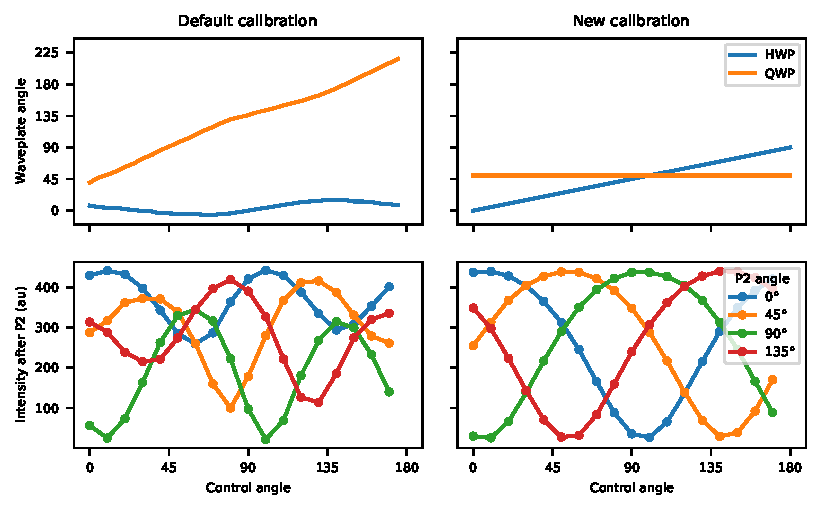
\includegraphics{detection_waveplate_calibrations.pdf}
	\caption{
		A comparison of the default detection waveplate calibration and the new one. The new calibration seems to actually rotate incident polarisation by an arbitrary angle.
	}
	\label{fig:detection waveplate calibrations}
\end{figure}




Second, I assessed both Abberior's and my calibration. As presented in \autoref{fig:detection waveplate calibrations}, my calibration works really well. However, changing P1 seems to mess up that idea. The detection waveplates seem to rotate the polarisation for P1 at \ang{0} or \ang{90}, but seem to circularise incoming light at \ang{45} and \ang{135} to a certain extent, such that the polarisation rotation is less effective. This needs to be fixed before we can confidently use polarisation-affecting elements in the detection path.

\begin{figure}[h]
	\centering
	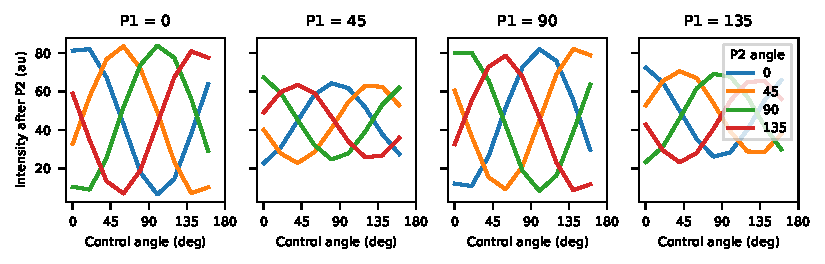
\includegraphics{p1_effects.pdf}
	\caption{
		The effect of rotating the incoming polarisation (P1). The detection waveplates seem to rotate the polarisation for P1 at \ang{0} or \ang{90}, but seem to circularise incoming light at \ang{45} and \ang{135} somewhat.
	}
	\label{fig:p1 effects}
\end{figure}

Third, I checked the POL cube, which seems to work as expected. \todo{Put figure in appendix.}

\section{Conventional polarisation microscopy: acquisition and analysis}
\label{sec:pol analysis}
 
Because the current setup offers so much control over the light polarisation on both the excitation and detection ends, one can perform polarisation microscopy in several different ways:
\begin{enumerate}
	\item Measuring the intensity of emission components parallel and orthogonal to linearly polarised excitation ($ I_\parallel $ and $ I_\perp $). This is a very established method of polarisation microscopy, and allows for making anisotropy images, where every pixel is calculated according to
	\begin{equation}
		r=\frac{I_\parallel - I_\perp}{I_\parallel + 2I_\perp}.
	\end{equation}
	
	\item Detection of emission polarised at different angles after circular polarisation.
	
	\item Detection of total emission intensity as a function of the polarisation angle of excitation light.
\end{enumerate}

Methods 1 and 2 require the PBS cube to be placed in one of the FC housings. When placed in FC1, the PBS cube reflects $ s $-polarised light (vertical) into APD1 and transmits $ p $-polarised light (horizontal) to be collected by APD2. Unfortunately, we cannot use these methods yet, since they rely on the action of the detection waveplates, even if they are not actively used during the acquisition. Once we do, however, the waveplates can be used to sample more than two angles during an acquisition. This is necessary to distinguish between light polarised along \ang{+-45}, since these two angles give exactly the same intensity when sampling at \ang{0} and \ang{90} degrees.

The last method, however, is not subject to those constraints, and is already achievable on the Tegenfeldt microscope. I have carried out some acquisitions and wrote some code for analysing this data. The process of acquiring and analysing these images goes as follows:
\begin{enumerate}
	\item Acquire a stack of images at different excitation polarisation angles $ \theta_n $. Then we have a three-dimensional array of intensity values $ I_{nxy} $.
	\item Align images in this stack with each other, as the excitation beam seems to move as a function of polarisation angle. The alignment algorithm will be explained later.
	\item Compensate for photobleaching.
	\item For every pixel, calculate the Fourier coefficient corresponding to a \ang{180}-periodic signal.
	\item Based on that information, construct a new image in the HSV (hue, saturation, value) colour space where pixel colour depends on the polarisation direction, the saturation shows the degree of polarisation and the brightness (value) shows the total intensity of a pixel. 

\end{enumerate}

\paragraph{Stack alignment.} Images in a stack are aligned using an ECC optimisation algorithm partly implemented in the OpenCV library \cite{Evangelidis2008}. The goal is to generate a new stack $ I'_{nxy} $ corrected for sample or beam drift. We will take the first frame as reference, setting 
\begin{equation}
	I'_{0xy} = I_{0xy}.
\end{equation}
For every other frame $ I_{nxy} $, we can calculate a warp matrix using the \texttt{findTransformECC()} method defined in OpenCV that maximises the correlation between $ I_{nxy} $ and $ I'_{(n-1)xy} $. We only calculate translational motion, so scaling and rotation are not allowed. Finally, we transform the original image using that warp matrix and \texttt{warpAffine()} and save the result as $ I'_{nxy} $, in other words:
\begin{equation}
	I'_{nxy} = \texttt{warpAffine}\left(
		I_{nxy}, 
		\texttt{findTransformECC}\left(I'_{(n-1)xy}, I_{nxy}\right)
	\right) \qq{for all} n>0.
\end{equation}

\paragraph{Bleaching compensation.} Since we want to calculate Fourier coefficient, we need to separate the photobleaching response from the polarisation response. We can do this by comparing two frames at identical polarisations and estimate the bleaching rate by their difference. Unfortunately, the Imspector software suite does not allow for rotating the excitation polarisation by more than \ang{175}, so we cannot do this exactly. We would be able to if we also used a PBS, but that is not an option, as explained before. Let $ \bar{I}_0 $ be the mean intensity of the first image, and $ \bar{I}_N $ the mean intensity of the last one. For now, we simply estimate the bleaching per frame as
\begin{equation}
	r = \sqrt[N]{\frac{\bar{I}_N}{\bar{I}_0}},
\end{equation}
given $ N+1 $ number of frames were acquired. Then we can compensate for photobleaching by multiplying every frame with a correction factor as
\begin{equation}
	I''_{nxy} = r^{-n} I'_{nxy}.
\end{equation}
This is far from perfect, but good enough for now.

\paragraph{Colouring the image.} For every pixel, calculate a complex-valued Fourier coefficient corresponding to a period of \ang{180} (at which we should see polarisation dependence) using
\begin{align}
	F_{xy} &= \sum_n I''_{nxy} e^{i2\theta_n}.
\end{align}
Then construct an image in the HSV (hue - orientation, saturation - degree of polarisation, value - total intensity) where 
\begin{align}
	h_{xy} &= \arg (F_{xy}),\\
	s_{xy} &= \abs{F_{xy}}/v_{xy},\\
	v_{xy} &= \sum_n I_{nxy}.
\end{align}
Finally, normalise these channels $ c $ to be in the range $ (0,1) $ and optionally apply a power law with a manually chosen coefficient $ \alpha_c $ for optimal visualisation,
\begin{equation}
	c'_{xy} = \left( \frac{c_{xy}}{\max (c_{xy})} \right)^{\alpha_c}.
\end{equation}
The effect of $ \alpha_c $ is presented in \autoref{sec:conventional pol}. If necessary, the Fourier image $ F_{xy} $ can be blurred before constructing a false colour image. This can be useful in high noise images.

\section{Polarisation-resolved STED microscopy (pSTED)}
\label{sec:methods psted}

Since polarisation is important to both excitation and emission of a fluorophore, it stands to reason that stimulated emission should also be polarisation dependent. In fact, that is what the calculation in Dyba et al.'s calculation of STED resolution is based on \cite{Harke2008, Dyba2005}. Moreover, excitation and stimulated emission are described by the same quantum mechanical process \cite{Foot}.

Would it then be possible to adapt the principle of conventional STED microscopy to increase the polarisation resolution of a microscope, instead of its spatial resolution? In this section, I will introduce a definition of polarisation resolution, a mathematical description of how this might be improved using pSTED, and how we adapted the microscope setup in order to achieve that. 

The general idea is that one can define a vectorial PSF (although a better term is photon fluence) that takes light polarisation into account. In a conventional polarisation microscopy setup, the probability of excitation of a fluorophore satisfies is proportional to $ \cos^2 \Delta $, where $ \Delta $ is the difference between the excitation polarisation and the transition dipole moment. This results in a FWHM resolution for conventional polarisation microscopy of 
\begin{equation}
	d_\theta = \ang{90}.
\end{equation}

\todo{This can also be seen from the fact that a cosine of any phase can be written as the sum of a cosine and a sine
\begin{equation}
	\cos(2\theta+\delta) = \cos\delta\cos 2\theta - \sin\delta\sin 2\theta.
\end{equation}
In other words: the sum of two cosines of a different phase }

By illuminating the sample with a depletion beam that is orthogonally polarised to the excitation laser, we can suppress fluorescence of fluorophores on the edge of this PSF, just like in conventional STED. This is illustrated in \autoref{fig:psted principle}.

\begin{figure}
	\centering
	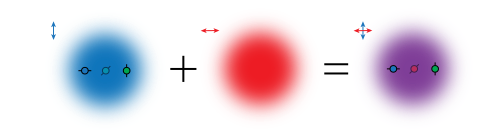
\includegraphics[width=\linewidth]{psted.ai}
	\caption{
		Illustration of the working principle of pSTED. The arrows outside indicate the polarisation of the laser light. The circles represent fluorophores with their transition dipole moment indicated by a line. The orthogonal polarisation of the depletion beam suppresses fluorescence of the fluorophore oriented at \ang{45}.
	}
	\label{fig:psted principle}
\end{figure}

\paragraph{Derivation of the pSTED PSF.} What follows is strongly inspired by Dyba et al.~\cite{Dyba2005}. Let $ \vb{x} = (x, y, z)$ be the spatial coordinates, $ \theta $ be an angle with the $ x $-axis in the $ xy $ plane (ranging from $ 0 $ to $ 2\pi$) and $ \phi $ be an angle with the $ z $-axis in the $ xz $ plane (ranging from $ -\pi $ to $+\pi$). We can also introduce a generalised coordinate $ \vb{y} = (\vb{x}, \theta, \phi) $, which will be useful later.

\todolist{
	\item Introduce proportionality constant $ A $. 
	\item Proper treatment of $ \phi $, but then say that we don't need to consider it to know what we want to know.
	\item Draw the parallel with normal diffraction limit better (kernels and convolutions)
}

Let the fluorophore population be described by the density $ \rho(\vb{y}) $. This function is normalised such that its integral is equal to the number of fluorophores. For example, a single fluorophore at the origin, pointing in the $ x $ direction with no out-of-plane tilt would be described by the Kronecker delta distribution $ \rho_0 = \delta(\vb{y}) $, which is defined as follows:
\begin{gather}
	\delta(\vb{y}) = 0 \qq{if} y\neq0, \\
	\int f(\vb{y})\delta(\vb{y}-\vb{y}_0) \dd{\vb{y}} = f(\vb{y}_0).
\end{gather}

The excitation beam is described by the electric field amplitude $ \vb{E}_\exc $, polarised along $ \theta_\exc $, and analogous for the depletion beam. Like \autoref{eq:convolution}, the emission intensity measured when the laser is focused on $ \vb{x} $ and polarised along $ \theta $, $ \phi $ is now some sort of a convolution integral, where we also have to integrate over the angles $ \theta $ and $ \phi $ like
\begin{equation}
	\begin{aligned}
		I_\emm 
			&= A \int 
				\sigma_\exc \abs{\unit{n}_{\theta'\phi'} \cdot \vb{E}_\exc(\vb{x}-\vb{x}')}^2 
				\rho(\vb{x}', \theta', \phi') 
				\dd{\vb{y}'} \\
			&= \int 
				\sigma_\exc I_\exc(\vb{x}'-\vb{x}) \abs{\unit{n}_{\theta'\phi'}\unit{n}_{\theta\phi}}^2
				\rho(\vb{x}', \theta', \phi') 
				\dd{\vb{y}'}
	\end{aligned}
\end{equation}
where $ \unit{n}_{\theta\phi} $ is a unit vector pointing in the direction of $ (\theta, \phi) $ and $ A = \epsilon_0c/2 $. The dot product can be expressed as
\begin{equation}
	\abs{\unit{n}_{\theta'\phi'}\unit{n}_{\theta\phi}}^2 = \cos^2\theta \cos^2\phi,
\end{equation}
so we can write that equation as a convolution product like
\begin{gather}
	I_\emm = (\rho*h_\exc)(\vb{y}),\qq{where} \\
	h_\exc(\vb{y}) = \sigma_\exc I_\exc(\vb{x}) \cos^2(\theta)\cos^2\phi.
\end{gather}
If we have a constant laser intensity $ I_\exc $ that is polarised along $ \theta $ (without any out-of plan polarisation), this would reduce to
\begin{equation}
	I_\emm = \sigma_\exc I_\exc \cos^2\theta_\exc
\end{equation}
for the distribution $ \rho_0 $. $ I_\emm $ is maximal when the excitation polarisation is in the $ x $ direction, as expected.

Now, we need to include the effect of the polarised depletion field, which amounts to adding an exponential factor under the integral
\begin{equation}
	I_\emm = A \int
		\sigma_\exc \abs{\unit{n}_{\theta'\phi'} \cdot \vb{E}_\exc(\vb{x}-\vb{x}')}^2  
		\exp(-\sigma_\dep \abs{\unit{n}_{\theta'\phi'} \cdot \vb{E}_\dep(\vb{x}-\vb{x}')}^2)
		\rho(\vb{x}', \theta', \phi') 
		\dd{\vb{y}'}.
	\label{eq:psted integral}
\end{equation}
In essence, we should then multiply the kernel $ h_\exc $ with the function $ \eta $
\begin{equation}
	h_\mathit{pSTED}(\vb{y}) = h_\exc(\vb{y}) \eta(\vb{y}) = \sigma_\exc I_\exc(\vb{x}) \cos^2(\theta) \exp(-\sigma_\dep I(\vb{x}) \sin^2 \theta),
\end{equation}
which assumes both electric fields are orthogonally polarised and confined to the $ xy $ plane. 

This model can easily be extended to account for depolarising effects such as rotational diffusion, energy transfer, et cetera. However, that is not necessary at this point. Instead, we would like to know the resolution improvement this gives us. With a little algebra, it can be shown that the the FWHM resolution satisfies
\begin{equation}
	d_\theta(I_\dep) = 2\arccos\sqrt\frac{\mathcal{W}\left(\frac{\sigma_\dep I_\dep e^{\sigma_\dep I_\dep}}{2}\right)}{\sigma_\dep I_\dep},
\end{equation}
where $ \mathcal{W} $ is the Lambert W-function. It is the inverse of the function $ f(x) = xe^x $. As expected, $ d_\theta(0)=\ang{90} $. $ d_\theta(0) $ is plotted in \autoref{fig:pol psf width}.

\begin{figure}
	\centering
	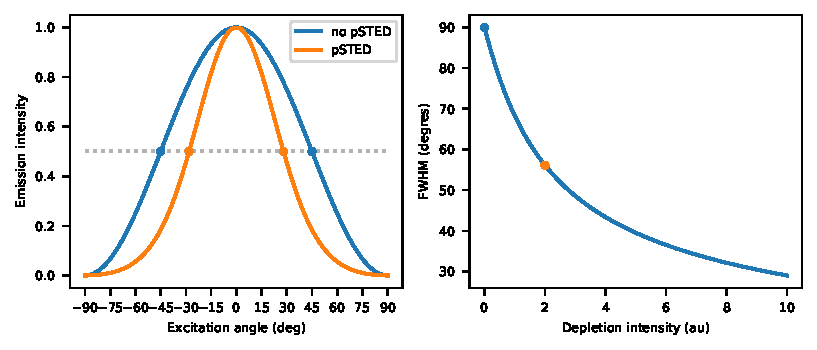
\includegraphics{pol_psf_width.pdf}
	\caption{
		\textbf{Left:} Narrowing of the fluorophore response as a result of a depletion field (of intensity $ I_\dep=2 $, as compared to the right pane). \textbf{Right:} The FWHM angular resolution $ d_\theta $ as a function of depletion intensity.
	}
	\label{fig:pol psf width}
\end{figure}

\paragraph{Implementation of pSTED.} The system was not set up for tuning the depletion polarisation. Instead, the STED polarisation is always circular, and this is ensured by a set of two fixed waveplates: a QWP and a HWP (refer to \autoref{fig:layout} and the description of the STED module in that section). 

To control the polarisation of the depletion beam, I first had to linearise the polarisation by compensating for the QWP in the beam path. That can be done by placing a QWP in the pSTED module in \autoref{fig:layout}. This works because 
\begin{equation}
	S_\qwp(\phi)S_\hwp(0)S_\qwp(-\phi) = R(2\phi).
\end{equation}
When the quarter-wave plates are aligned like that, this system simply rotates the polarisation by a fixed angle. Then, adding a HWP before this setup suffices to get full control over the polarisation angle of the depletion beam.

\section{Samples}
\label{sec:samples}

During the project, samples were very generously provided by research groups led by Pontus Nordenfelt and Vinay Swaminathan (Division of Infection Medicine, Faculty of Medicine, Lund University).

Results of the cell sample shown in the experimental section contain a human cell line infected with bacteria of the Yersinia genus. Stainings present are: DAPI (nucleus), GFP (bacteria) and SiR-actin. SiR-actin is an organic molecule (silicon-rhodamine) rigidly linked to an actin monomer. This dye is perfect for our setup, as SiR can be excited at 664~nm and has an sufficient absorption cross-section at 775~nm to perform STED. In addition, the fact that it is rigidly bound to the actin cytoskeleton means the light it emits is strongly polarised and reports on the the actin filament orientation.

I also used two control samples for calibration measurements. The first is a sample of small \question{How small?} reflective gold colloids, which were used to image the laser point spread functions. The second contains larger Tetraspec fluorescent beads (Invitrogen).
	% !TeX spellcheck = en_GB
\chapter{Results}

\section{Conventional polarisation microscopy}
\label{sec:conventional pol}
\begin{figure}
	\centering
	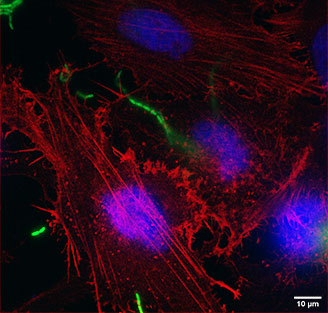
\includegraphics[width=.5\linewidth]{composite.jpg}
	\caption{
		Composite view of a Yersinia sample, labeled with phalloidin instead of actin. Blue: DNA (DAPI). Green: bacteria (GFP). Red: actin (phalloidin).
	}
	\label{fig:composite}
\end{figure}

SiR has been reported to be suitable for STED microscopy with excitation at 640~nm and depletion at 775~nm \cite{DEste2015}, so we would expect the SiR-actin stained sample to behave well in our setup too. The effect of the depletion laser (in conventional, i.e.~donut mode) is presented in Figures \ref{fig:ssted} and \ref{fig:ssted supplementary}. When zoomed in (\autoref{fig:ssted supplementary}), it becomes visible that the fibres are not uniformly stained as individual fluorophores become apparent.

\begin{figure}
	\centering
	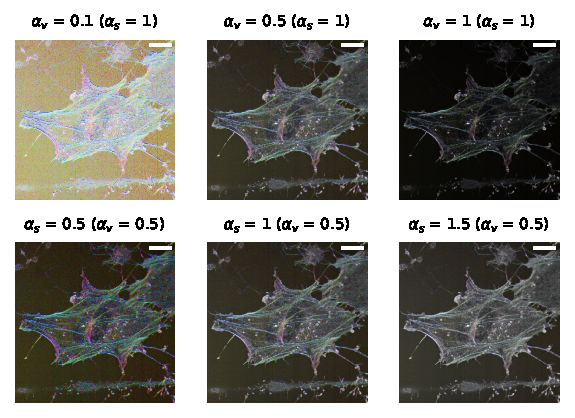
\includegraphics{conventional_pol.pdf}
	\caption{
		Polarisation microscopy images of three different cells. The colour wheel indicates the direction of polarised light corresponding to a certain colour. Scale bars \SI{10}{\mu m}. 
	}
	\label{fig:conventional pol}
\end{figure}

\begin{figure}
	\centering
	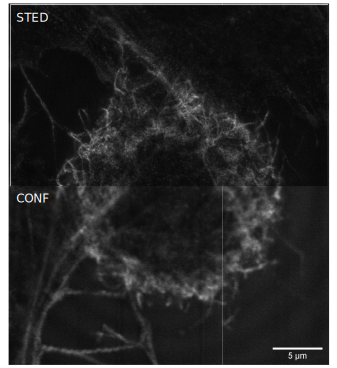
\includegraphics{ssted_2.pdf}
	\caption{
	 stained with SiR-actin, in confocal mode (bottom) and with the STED laser at 15\% power (top). More FOVs are displayed in \autoref{fig:ssted supplementary}.
	}
	\label{fig:ssted}
\end{figure}

Even though we can't use polarisation on the detection side yet, it is already possible to obtain polarisation-resolved images by varying the angle of excitation polarisation. As a proof of concept, I imaged the sample described in \autoref{sec:samples}, stepping the excitation light from \ang{0} to \ang{170} in steps of \ang{10}. Applying the algorithm detailed in \autoref{sec:pol analysis} to three different ROIs resulted in \autoref{fig:conventional pol}. As expected, vertically oriented fibres are excited by horizontal polarisation \cite{Spira2017}.
I also included power law scaling of the saturation (degree of polarisation) and value (total brightness) in the visualisation algorithm. These serve to adjust the brightness and contrast of the figure, as shown in \autoref{fig:power law exponents}.

I also tried to get polarisation images at STED resolution. Unfortunately, STED microscopy is quite taxing on the sample and results in strong photobleaching, which limits the number of points at which the excitation polarisation can be sampled (see \autoref{fig:ssted pol}). There is a qualitative difference between the intensity profile of two ROIs that contain orthogonally oriented actin fibres. In particular, the maximum of one is located at \ang{45} (after subtracting an exponential photobleaching response), while the other shows a maximum around \ang{135}. The quality of this particular image is unfortunately not sufficient to colour it as we did in \autoref{fig:conventional pol}.

In short, this section shows that we have successfully implemented conventional polarisation microscopy on the microscope setup and that SiR-actin is a suitable fluorophore to conduct research in Yersinia samples. There are two main limitations at the moment: the detection waveplates are not calibrated correctly, so we cannot use polarisation in the detection pathway, and the trade-off between spatial resolution and polarisation information requires special care.

\begin{figure}
	\centering
	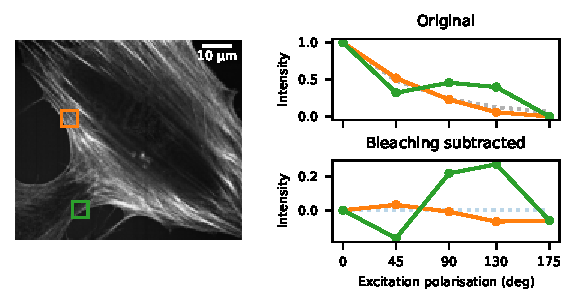
\includegraphics{ssted_pol.pdf}
	\caption{
		\textbf{Left:} First frame of a polarisation acquisition series, with two ROIs indicated that contain fibres of roughly perpendicular orientation. \textbf{Top right:} Integrated intensity of those ROIs at different sample points, normalised to the intensity present in the first frame. Dashed line: best-fit exponential curve. \textbf{Bottom right:} Same as top right, but with the exponential subtracted.
 	}
 	\label{fig:ssted pol}
\end{figure}

\section{pSTED}

After implementing the pSTED optics in \autoref{sec:psted implementation}, I will discuss the results we have so far. To verify that stimulated emission is polarisation-dependent, we imaged isotropic fluorescent beads under two different conditions. In the first condition, the beads were excited with vertically polarised light and depleted by a laser polarised along different angles and at different power levels. Regardless of the angle, the fluorescence signal drops as the depletion power is increased, but the rate at which depends on the depletion polarisation. The depletion rate is highest when the lasers are aligned and lowest when they are orthogonal. This result can be explained by photoselection. When an isotropic sample is excited by linearly polarised light, fluorophores with a dipole moment orthogonal to the excitation beam will not be excited. As a result, the average excited fluorophore's transition dipole is oriented parallel to the excitation polarisation. Since depletion is most effective when the depletion polarisation is aligned with the fluorophore (as predicted by \autoref{eq:psted integral}) in this case that also means it is most effective when aligned with the excitation laser. We did indeed observe this effect, see \autoref{fig:psted beads} (Left). 

On the other hand, if the sample is excited with circularly polarised light, the rate of depletion should not depend on the depletion polarisation. I performed this experiment twice. The first time, I imaged an ROI at different depletion powers before I changed the depletion polarisation (\autoref{fig:psted beads}, Middle). The second time, I imaged ROIs at different depletion polarisations before I changed the depletion power (\autoref{fig:psted beads}, Right). While the results are substantially different from the linear polarisation case, it would be a stretch to claim that they clearly show that the fluorescence decay is independent of the depletion polarisation. I believe that they do, but more research is required, perhaps by simply running the experiment several times to decrease noise in the experiment. (Note that it was much easier to automate the acquisition of the linear polarisation data. As such, the figure shown is an average of five runs, while the others only show data of a single run.)

\begin{figure}
	\centering
	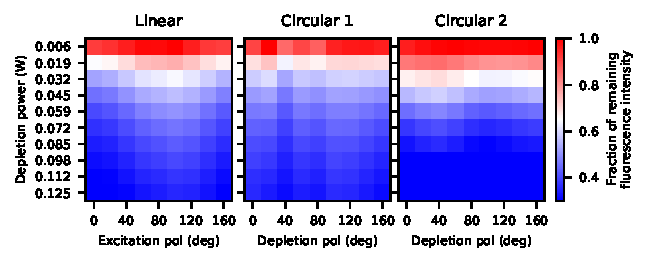
\includegraphics{psted_beads.pdf}
	\caption{
		Dependency of surviving fluorescence on intensity and polarisation of depletion beam. \textbf{Left:} linearly polarised excitation at 0° (vertical). \textbf{Middle:} circularly polarised excitation (measurements taken by column). \textbf{Right:} circularly polarised excitation (measurements taken by row).
	}
	\label{fig:psted beads}
\end{figure}

Even though they could be improved, the results do show that depletion efficiency seems to be dependent on the polarisation of the depletion laser and the orientation of the fluorophore, so pSTED is likely to work. Next, we performed this experiment on a cell sample, but since the actin fibres are not isotropic, we did not need to use linearly polarised excitation to select a subset of fluorophores. Instead, we imaged several fibres with circularly polarised excitation light and manipulated the depletion angle to assess whether it was possible to perform pSTED on a biological sample, see \autoref{fig:psted scans}. Without a depletion laser, all we can see is photobleaching. With a depletion laser, the photobleaching response disappears and is taken over by a signal that depends on the depletion polarisation (orange). Although more research is needed, this shows that pSTED could be a valuable new tool in the polarisation microscopy field.

\begin{figure}
	\centering
	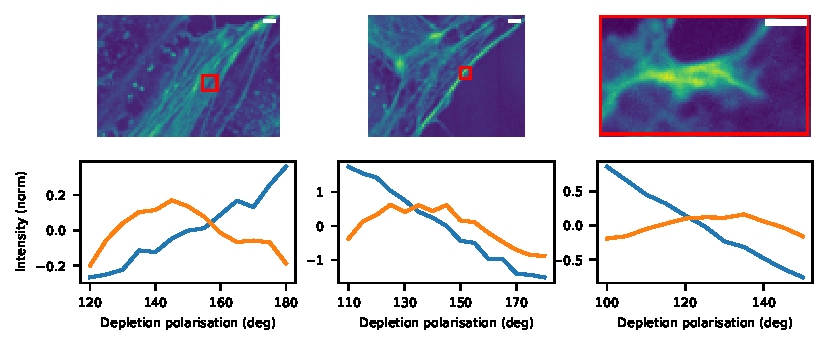
\includegraphics{psted_scans.pdf}
	\caption{
		When samples are excited with circularly polarised light, the polarisation of the depletion beam can modulate the fluorescence intensity. \textbf{Top:} FOVs with a marked ROI in red. Scale bars \SI{2}{\mu m}. \textbf{Bottom:} Intensity profile, as a function of depletion polarisation. Orange: depletion beam turned on. Blue: depletion beam turned off. \todo{column layout for figure}
	}
	\label{fig:psted scans}
\end{figure}





























	% !TeX spellcheck = en_GB

\chapter{Outlook}

Finally, I will review my findings and thoughts on follow-up research.

Firstly, we have achieved polarisation microscopy on the Tegenfeldt STED microscope, and with that reached the main goal of this thesis project. We are technically able to perform polarisation microscopy at confocal resolution and overlay the structure found by non-polarised STED micrographs taken on the same setup. This is already a great result. We have also established that SiR-actin is a probe that is suitable for our setup: it is excited at 640~nm, it is efficiently depleted by the 775~nm laser and its bond to actin is sufficiently rigid for polarisation microscopy.

There is some work left to do before results on biological specimens are ready to be published, however. Firstly, the calibrations of the microscope can be improved. The 640~nm laser is not as well polarised as the 561~nm one is, despite going through a similar set of optics. The circularity of the STED polarisation can also be improved. Secondly, the waveplates of both excitation lasers rotate more than necessary when the laser polarisation is rotated during a polarisation scan. Improving this point should increase the acquisition speed and polarisation quality. Thirdly, we need a quantitative understanding of the depolarising effects of different components instead of a qualitative one. This knowledge may then be used for correcting and interpreting the raw data. We should image a sample in our setup and that of another research group and compare the results quantitatively. When successful, the setup is ready to produce publication-quality polarisation microscopy results.

Secondly, there is some other ground to be gained on the conventional polarisation microscopy front: in the detection waveplates. Once these are properly aligned, it becomes possible to use a polarising beam splitter in the detection pathway, which gives twice the amount of orientational information in a single acquisition. This is great for experiments that are limited by the photon budget: very sensitive samples can then be imaged with polarisation at confocal resolution, or less sensitive ones could be imaged at STED resolution.

Thirdly, we should continue developing pSTED. The results so far are promising, but have not yet demonstrated the full potential of this method. This is due in part to finding the right balance between angular resolution and photodamage due to the increased depletion power. This problem is exacerbated by the fact that having a higher angular resolution requires acquiring more frames on top of a high depletion power. Now that we know pSTED is likely to be possible with these SiR-actin samples, we should get a fresh sample and measure the polarisation signature of actin micropatterns. On the more practical side of things, there are two obvious improvements that can be made: running the cabling to the HWP rotator stage through the back of the optical box and integrating the HWP into the microscope control software to automate pSTED acquisitions.

Finally, this setup offers some other possibilities that have not yet been discussed in this thesis, and there's a lot of methods where we can use fluorescence polarisation. Using the fluorescence lifetime imaging (FLIM) module, it is possible to quantify the rotational diffusion of a fluorophore by assessing how its polarisation signal changes on a timescale of nanoseconds. It is also possible to quantify fluorescence resonant energy transfer (FRET) between fluorophores by measuring the depolarisation effect the sample has on incoming light. Another possibility is to apply these results to other research programmes in the Tegenfeldt group: polarisation microscopy should be able to quantify the degree of polarisation of DNA flowing through a microfluidic device, such as a DLD (deterministic lateral displacement) chip.

\appendix

	\bibliographystyle{mystyle}
	\bibliography{other_sources,mendeley}
	
	% !TeX spellcheck = en_GB
\chapter{Acknowledgements}

Many thanks to Jason and Jonas for their great supervision. You have taught me so much, both academically and personally, and I feel extremely lucky that I got to do my thesis project with you guys. Thanks also to the others in the Tegenfeldt group: Elham, Esra, Oskar and Bao, for the good vibes and the occasional helping hand.

I am grateful to our collaborators in the Nordenfelt and Swaminathan groups, particularly to Valeriia, Swathi and Oscar who provided the samples I used throughout my project. To the polarisation community in Lund at large: thank you. I am grateful for the opportunity to organise our discussion sessions, which turned out the be instrumental to several parts of my thesis project.

A special mention goes out to Carl Troein. He has not been directly involved in this project, but as my programme coordinator, he has helped me navigate my new university and its administrative system and has helped me out a ton with getting a summer internship, which turned out to be a stepping stone to my next challenge.

I want to thank my friends and family for the continued support they gave me during this project, and simply for being part of my journey. Finally, I want to thank the Swedish public in general. I am extremely grateful for the opportunity to live in and discover your country for the past two years. It's been a blast!
%If there's anything I've learnt from my time here, it's this: \emph{det finns inget dåligt väder, bara dåliga kläder}.

\bigskip

\noindent Jonas, I promised you I'd share my star recipes, so check out the next page.
\newpage
\section*{Misir Wat}
\paragraph{Ingredients}
\begin{itemize}
	\item 4 tablespoons butter (or niter kibber, that's even better)
	\item 1 large yellow onion, very finely diced
	\item 3 cloves garlic, finely minced
	\item 1 tomato, very finely chopped
	\item 3 tablespoons tomato paste
	\item 2 tablespoons berbere , divided (you can get this at African Daily Market in Lund)
	\item 1 cup red lentils, rinsed
	\item 2.5 cups of vegetable stock
	\item 1 teaspoon salt
\end{itemize}

\paragraph{Preparation}
Melt 3 tablespoons of the butter in a medium stock pot.  Add the onions and cook over medium-high heat for 8-10 minutes until golden brown.  
Add the garlic, tomatoes, tomato paste and 1 tablespoon of the berbere and cook for 5-7 minutes. Reduce the heat if needed to prevent burning.
Add the broth and salt, bring it to a boil, reduce the heat to low and cover and simmer the lentils, stirring occasionally, for 40 minutes (adding more broth if needed) or until the lentils are soft.
Stir in the remaining tablespoon of butter and berbere. Simmer for a couple more minutes. Add salt to taste.
Serve with Ethiopian injera, sourdough bread, or rice.

Source: \href{https://www.daringgourmet.com/misir-wat-ethiopian-spiced-red-lentils/}{\texttt{daringgourmet.com}}

\section*{Ginger Beer}

To start a ginger bug, combine 0.5 litres of water, 20 g of ginger (chopped or grated, but not peeled), and 28 g sugar in a glass pot. Cover it with a clean towel and keep it at room temperature. Until it becomes fizzy, add 20 g of ginger and 30 g of sugar every day.

Then, combine 2 L of water, 200 g of sugar, and 75 g of ginger in a pot. Bring it to a boil, then reduce the heat and simmer for 5 to 8 minutes. Take it off the heat and let it cool down to room temperature. Add 100 g of strained ginger bug, and optionally some spices and the juice of three lemons. Divide over some airtight bottles and keep those at room temperature. Burp them daily by opening the cap to release built-up gas for about a week until the flavour is right and they are very carbonated. Then store them in the fridge for at least a couple of hours and enjoy!

Source: \href{https://www.joshuaweissman.com/post/fermented-ginger-beer}{\texttt{joshuaweissman.com}}

	\chapter{Code and data availability}

I've spent quite a bit of effort ensuring this entire thesis easily reproducible from the raw data. To that end, the source code and data necessary to produce this file and the figures in it are published on GitHub, at \url{https://github.com/wduverger/msc-thesis}. 
If you experience any trouble getting the code to run, have any questions regarding this thesis or just want to chat about polarisation microscopy in general, please reach out! I am always happy to help.
	% !TeX spellcheck = en_GB

\chapter{A note on laser safety}

The \SI{775}{nm} line is a class 4 laser source. Under normal operation, the user is protected from it. However, when calibrating the STED beam or placing new components in the beam path, it is theoretically possible for the collimated laser beam to be reflected into the user's eyes. A high-powered laser beam can do permanent damage to the skin and retina, so we have to make sure we stay below the limits imposed by the Work Environment Agency's (Arbetsmiljöverkets) limits \cite{AFS2009:7}. These regulations set forth three main conditions to calculate the Maximum Permissible Exposure (MPE) of a pulsed laser, see table 2.6 of the regulations. Important values and formulas about our setup, as well as the limits provided by the Work Environment Agency are provided in \autoref{tab:laser-safety} and in the text below.

\begin{table}[h]
	\centering

	\begin{tabular}{lll}
		\toprule
		Quantity                   & Symbol               & Value                 \\ \midrule
		\multicolumn{3}{l}{\textbf{Laser operating characteristics}}              \\
		Beam radius                & $ r $                & 0.5 mm                \\
		Pulse width (FWHM)         & $ \tau $             & 1.3 ns                \\
		Pulse repetition frequency & $ f $                & 40 MHz                \\
		Pulse energy               & $ E_\mathit{pulse} $ & 31 nJ                 \\
		Average power              & $P_\mathit{avg} $    & 1.25 W                \\
		                           &  \\
		\multicolumn{3}{l}{\textbf{Safety parameters}}                            \\
		Thermal correction time    & $ T_\mathit{min} $   & 18 \si{\micro\second} \\
		Ca                         & $ C_a $              & 1.41                  \\
		Cc                         & $ C_c $              & 1                     \\
		Ce                         & $ C_e $              & 1                     \\ \bottomrule
	\end{tabular}	
	\caption{Operating characteristics of the 775 laser line and relevant safety parameters. }
	\label{tab:laser-safety}
\end{table}

\paragraph{Rule 1: The dose of a single pulse must not exceed the single-pulse MPE.} The pulse dose $ H_\mathit{pulse} $ of the 775~nm laser at full power is
\begin{equation}
	H_\mathit{pulse} = \frac{E_\mathit{pulse}}{2\pi r^2} \approx \SI{39}{mJ/m^2},
\end{equation}
whereas the MPE equals
\begin{equation}
	H_\mathit{pulse}^\mathit{MPE} = \num{5e-3} C_a C_e = \SI{7.1}{mJ/m^2}.
\end{equation}
This formula is found in table 2.2 of the regulations.

\paragraph{Rule 2: The dose of a single pulse may not exceed the thermally-corrected MPE.} This weighs the pulse MPE with the amount of pulses in an interval $ T_\mathit{min} $. The number of pulses in such an interval is $ n = f\cdot T_\mathit{min} $, so
\begin{equation}
	H_\mathit{thermal}^\mathit{MPE} =  n^{-1/4} H_\mathit{pulse}^\mathit{MPE} = \SI{1.3}{mJ/m^2}.
\end{equation}
Rule 2 is therefore more strict than the rule 1. For safe operation, the laser must be ran at a power below 3.3\% $ (=H^\mathit{MPE}_\mathit{thermal} / H_\mathit{pulse}) $.

\paragraph{Rule 3: The cumulative dose for a group of pulses in an interval of time t must not exceed the MPE for a single pulse of that time.} Taking the necessary values from tables 2.2 and 2.3 of the regulations, the cumulative MPE is defined as
\begin{equation}
	H_\mathit{tot}^\mathit{MPE}(t) = \left\{\begin{array}{rl}
		\num{5e-3} \:C_a C_e &  t<\SI{18}{\mu s,} \\
		18 t^{0.75} \:C_a C_e &  \SI{18}{\mu s} < t < \SI{10}{s}, \\
		10 t\:C_a C_c  &t> \SI{10}{s}.
	\end{array}\right.
\end{equation}
The actual dose, on the other hand, is
\begin{equation}
	H_\mathit{tot}(t) = \lfloor ft \rfloor H_\mathit{pulse},
\end{equation}
where $ \lfloor \cdot \rfloor$ is the flooring function. This function is plotted in \autoref{fig:laser-safety-mpe}, from which it can be seen that the laser is only safe to use at 0.0005\% capacity. Since the minimum laser power offered by the software is .05\%, OD2 goggles should be worn to guarantee safe operation of the 775~nm laser.

\begin{figure}
	\centering
	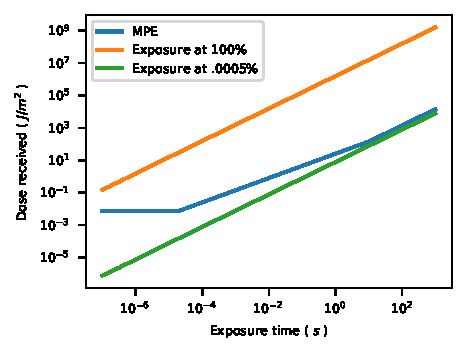
\includegraphics{laser_safety.pdf}
	\caption{Maximum permissible  and actual exposure to the collimated STED beam as a function of exposure time.}
	\label{fig:laser-safety-mpe}
\end{figure}
	% !TeX spellcheck = en_GB
\chapter{Supplemental figures}


\begin{figure}[ht]
	\centering
	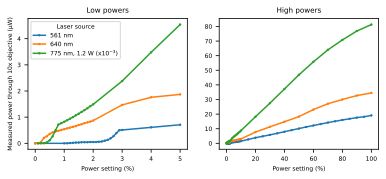
\includegraphics{laser_power}
	\caption{
		The power of each of the three lasers as measured through a 10x objective. Notice the non-linearity at low power settings. The 775 nm data was scaled down by three orders of magnitude.
	}
	\label{fig:laser power}
\end{figure}

\begin{figure}
	\centering
	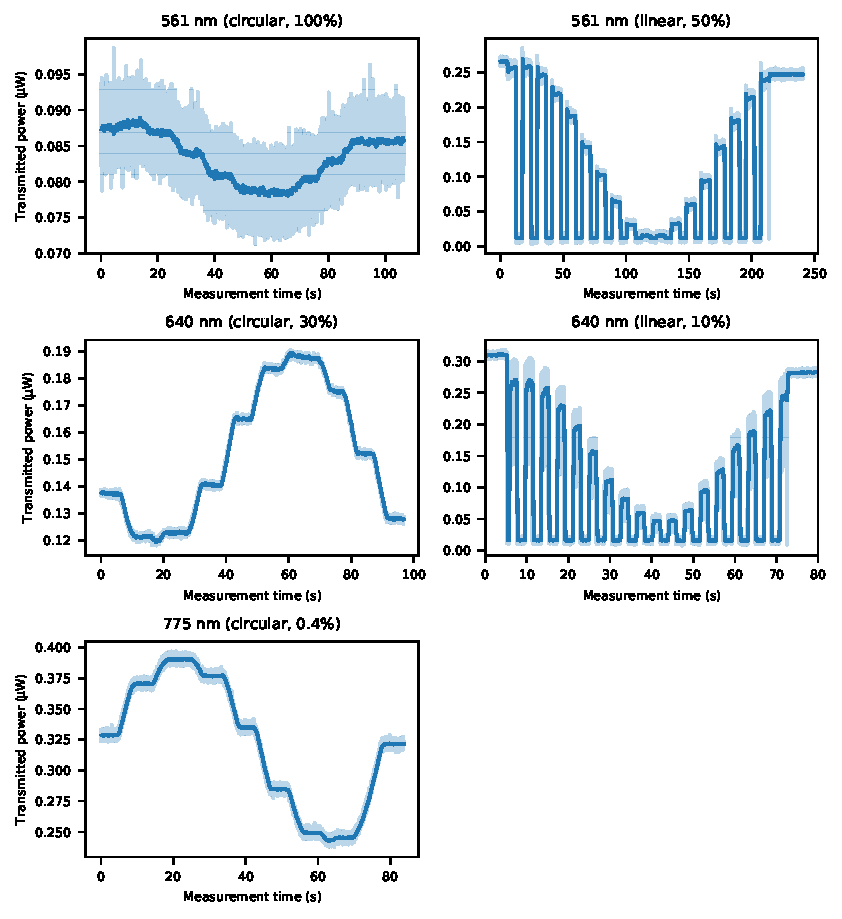
\includegraphics{laser_polarisation}
	\caption{
		Polarisation characterisation of the different lasers. To characterise circular polarisation, a polariser was placed in the sample and scanned from \ang{0} to \ang{180} in steps of \ang{20} (notice that I forgot to sample \ang{260} in the 775 nm data). Linear polarisation was characterised by fixing the polariser in place at \ang{0} and scanning the laser itself from \ang{0} to \ang{180} in steps of \ang{10}. Dark blue: average over 200 samples, light blue: raw data.
	}
	\label{fig:laser polarisation}
\end{figure}

\begin{figure}
	\centering
	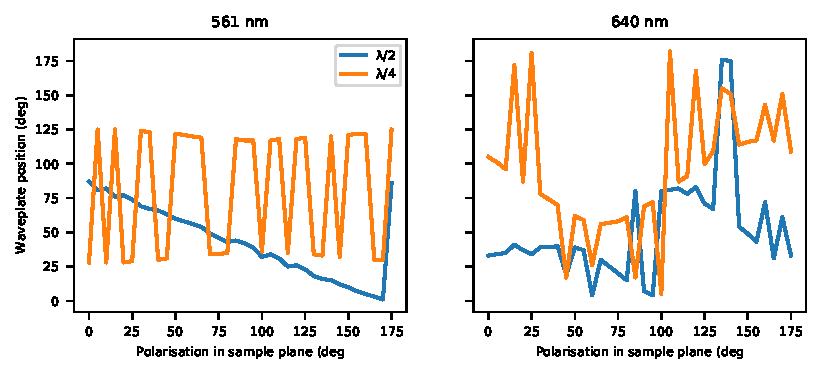
\includegraphics{excitation_waveplate_calibrations.pdf}
	\caption{
		Calibrations of the excitation waveplates, as supplied by the microscope manufacturer.
	}
	\label{fig:excitation waveplate calibration}
\end{figure}

\begin{figure}
	\centering
	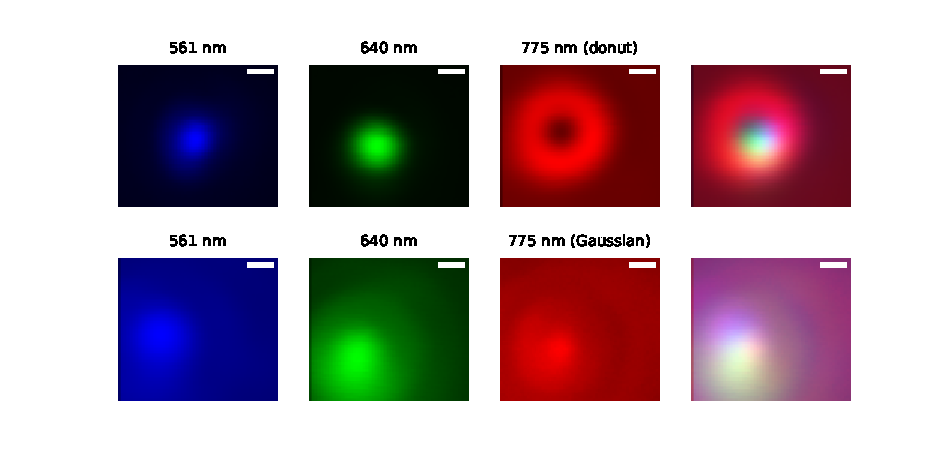
\includegraphics{laser_psfs.pdf}
	\caption{
		Point spread functions of the different lasers (in donut and Gaussian modes) at different SLM configurations, by measuring the reflection from 100 nm wide gold beads. Scale bars 200 nm.
	}
	\label{fig:normal psfs}
\end{figure}

\begin{figure}
	\centering
	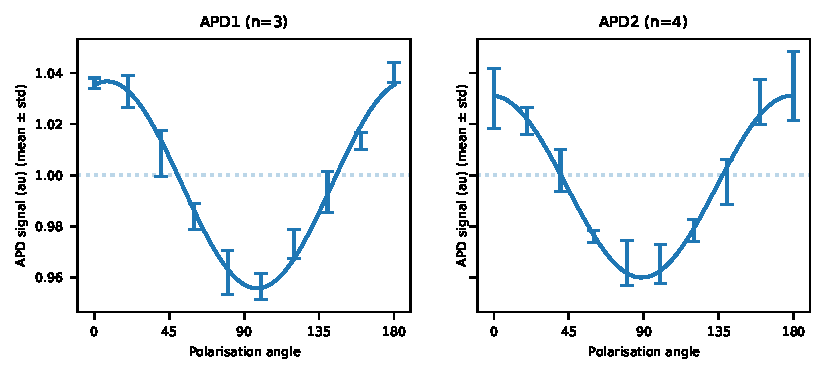
\includegraphics{apd_pol_sensitivity.pdf}
	\caption{Dependence of the signal from APD1 on the angle of polarisation of incoming light.}
	\label{fig:apd pol sensitivity}
\end{figure}

\begin{figure}
	\centering
	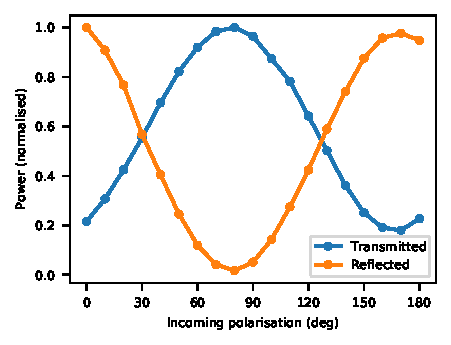
\includegraphics{pol_cube.pdf}
	\caption{Performance of the polarising beam splitter.}
	\label{fig:pol cube}
\end{figure}

\begin{figure}
	\centering
	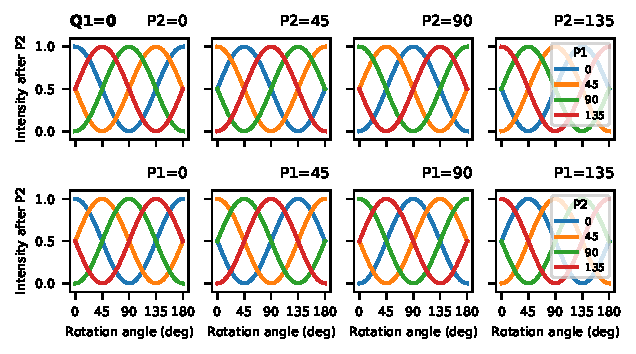
\includegraphics[scale=.95]{p1_effects_qwp_aligned.pdf}
	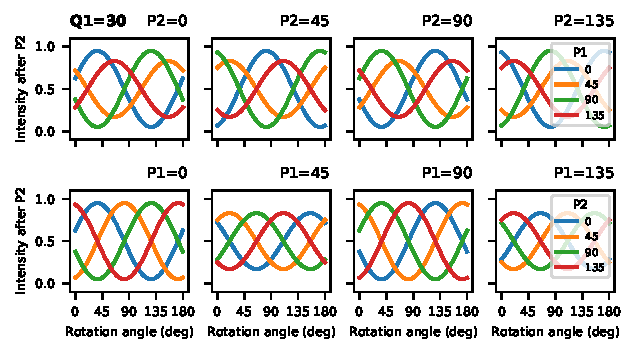
\includegraphics[scale=.95]{p1_effects_qwp_30.pdf}
	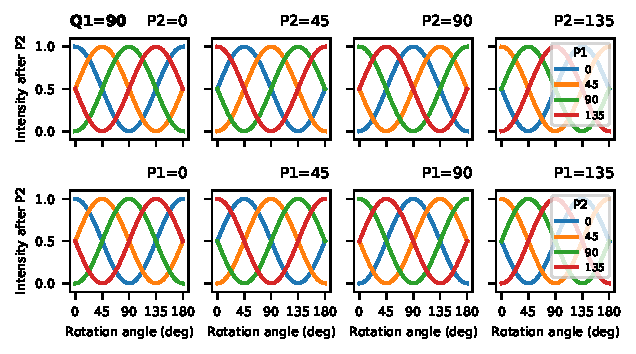
\includegraphics[scale=.95]{p1_effects_qwp_90.pdf}
	\caption{
		Simulation of the effect of QWP alignment on the action of the detection pathway. Shown are three simulations in which the first QWP is rotated by 0, 30, and 90 degrees, respectively. The second QWP is always rotated by 0, and the HWP is rotated to half the rotation angle (x-axis). When the QWPs have an offset of 90 degrees (bottom), the upper and lower panels (with either P1 or P2 constant) are identical, but when they are aligned (top), there is a phase difference. When they are not aligned at all (middle), intensity variations are prominent. This simulation is based on \autoref{eq:detection waveplates}.
	}
	\label{fig:detection waveplate simulations}
\end{figure}

\begin{figure}
	\centering
	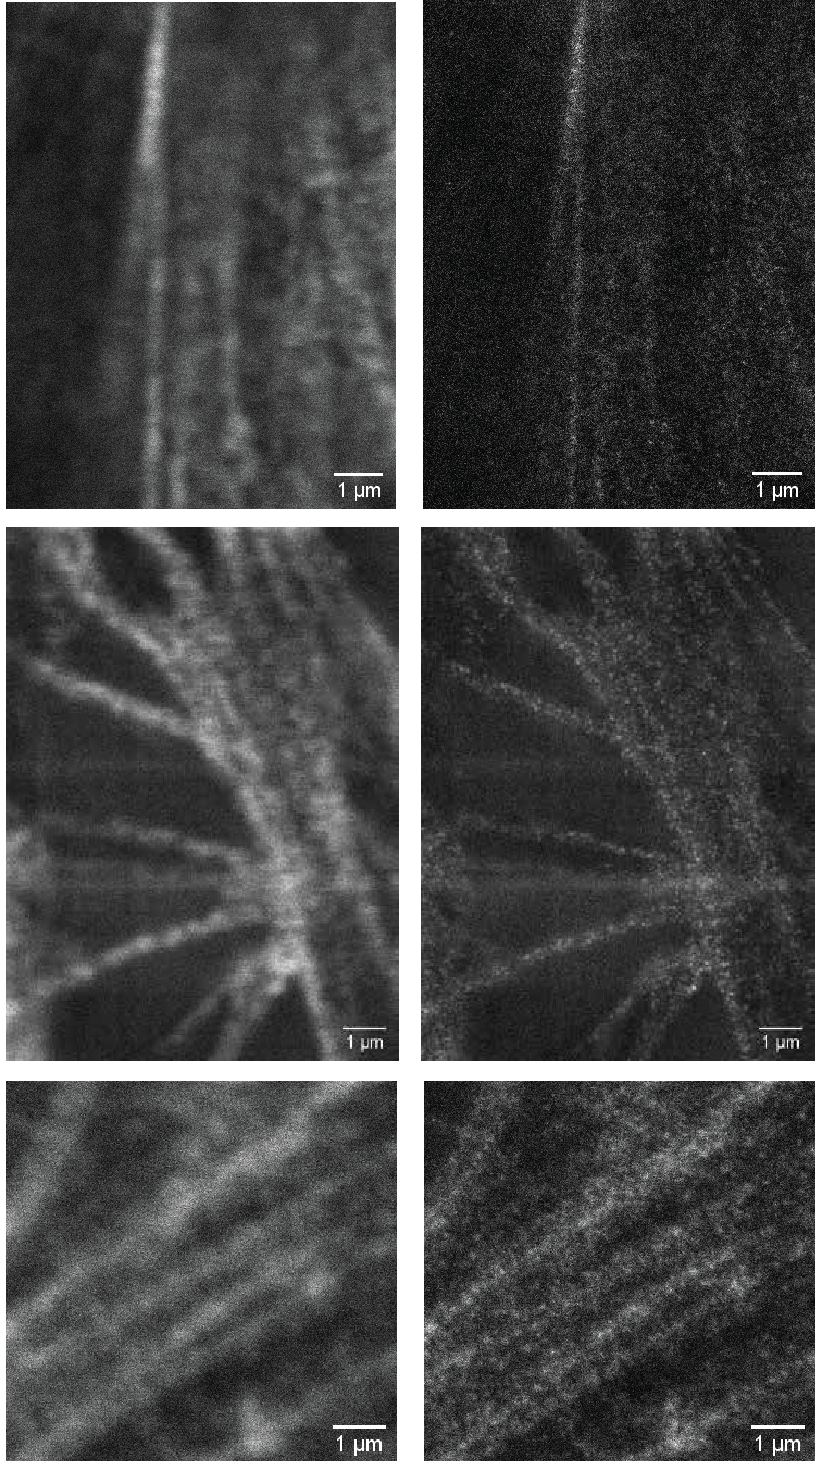
\includegraphics[width=.8\linewidth]{ssted_1.pdf}
	\caption{
		Confocal (left) and STED (right) acquisitions of various fields of view.
	}
	\label{fig:ssted supplementary}
\end{figure}


\begin{figure}
	\centering
	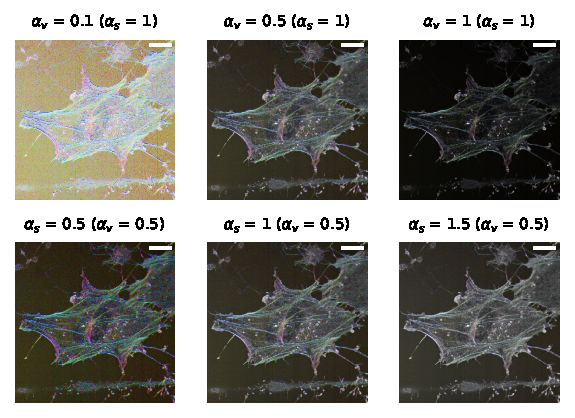
\includegraphics{conventional_pol.pdf}
	\caption{
		The effect of the exponents $ \alpha_s $ (tuning saturation) and $ \alpha_v $ (scaling brightness) on an image.
	}
	\label{fig:power law exponents}
\end{figure}

\begin{figure}
	\centering
	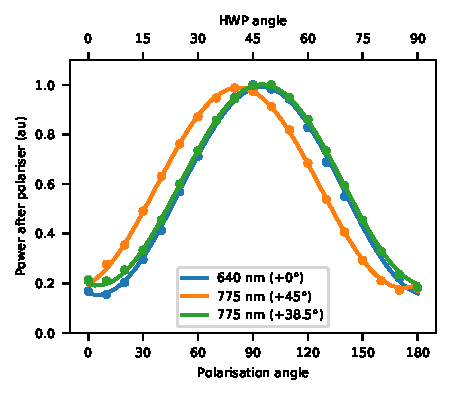
\includegraphics{psted_hwp_offset.pdf}
	\caption{
		The rotating HWP I put in the beamline controls the depletion beam polarisation. With an offset of 38.5°, the depletion beam is parallel to the 640 laser (set to vertical linear polarisation).
	}
	\label{fig:psted hwp offset}
\end{figure}

\begin{figure}
	\centering
	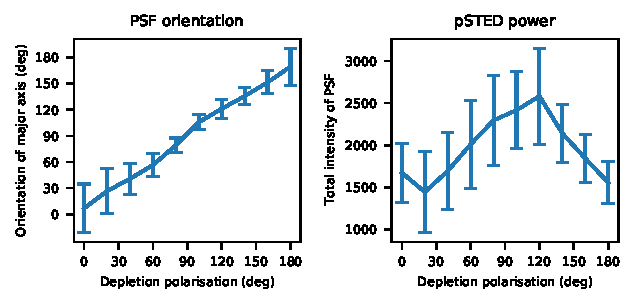
\includegraphics{psted_psfs_orientation_and_power.pdf}
	\caption{
		\textbf{Left:} The pSTED PSF is elliptical, and its orientation matches the light polarisation. \textbf{Right:} pSTED intensity depends on polarisation. Error bars show standard deviation, n=10.
	}
	\label{fig:psted psf orientation and power}
\end{figure}

\begin{figure}
	\centering
	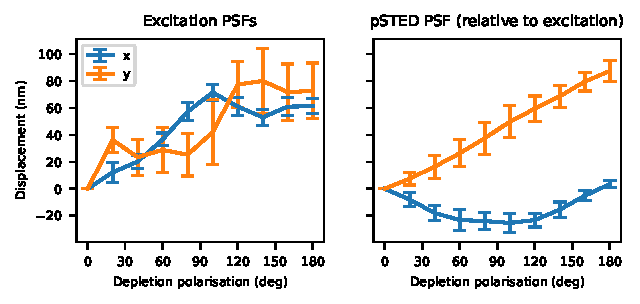
\includegraphics{psted_psfs_displacement.pdf}
	\caption{
		The displacement of the laser PSFs as a function of depletion polarisation. \textbf{Left:} The displacement of the 561~nm and 640~nm PSFs (representing drift in the image). \textbf{Right:} Displacement of the pSTED PSF relative to the excitation PSFs.
	}
	\label{fig:psted displacement}
\end{figure}

\end{document}